\marginpar{Meine Lebenserinnerungen im Abriss von 1930 --}
Meine sommerlichen Urlaubswochen in Oberitalien hatten einen Einfluss auf meine politischen Anschauungen. Ich gelangte allmählich zu der Meinung, dass ein dem italienischen Faschismus ähnliches Regime unter Hitler und Männern wie Gregor Strasser u.a. Deutschland aus der parlamentarischen (32 Parteien!) und wirtschaftlichen (fast 7 Millionen Arbeitslose) Krise heraushelfen könnte.

Hitlers Auftritt im September 1930 in der überfüllten Breslauer Jahrhunderthalle beeindruckte mich positiv. National und sozial -- diese Parole fand ich zeitgemäß. Sein Buch \enquote{Mein Kampf} forderte zwar meine Kritik heraus, ich glaubte jedoch, es handle sich hier um eine Propagandaschrift eines tüchtigen Politikers, der zunächst einmal an die Macht kommen wolle und sich dann maßvoll zeigen werde, auch im Kampf gegen das Judentum. So meinte ich, sein Kampf werde sich vor allem gegen die nach 1918 aus dem Osten, besonders Galizien, Weißrussland und Polen hereingefluteten Juden, nicht aber gegen in Deutschland alteingesessene und z.T. sehr verdiente jüdische Staatsbürger richten. An Mitgliedschaft in der \ac{nsdap} dachte ich umso weniger als diese den Beamten bis zum Tage der Machtübernahme am 30.1.1933 verboten war. Aus meiner Gesinnung machte ich jedoch weder im Kollegium noch in den Klassen -- trotz aller gebotenen Vorsicht -- kein Hehl. Meine schulische Arbeit fand allmählich Anerkennung, so bei Reifeprüfungen in Französisch und Deutsch beim Vorsitzenden (\enquote{Ihre Prüfungen haben beachtliches Niveau}) und gelegentlich einer dienstlichen Besprechung sagte mir Stadtschulrat Dr. Lauterbach, er freue sich, in mir einen der besten Lehrer des Elisabethgymnasiums zu sehen. Bei meinen Abiturientengutachten -- damals wurden vom Klassenleiter ausführliche Charakteristiken, die in der Regel etwa 3 Quartseiten umfassten, verlangt -- halfen mir meine gründlichen charakterologischen Studien, die sich auf das Gebiet der wissenschaftlichen Graphologie erstreckten.

Mein Direktor Dr. Lillge übertrug mir Rede- und Feiergestaltung der Goethefeier im Jahr 1932, ich lehnte jedoch ab, da ich mich einer solchen Aufgabe nicht gewachsen fühlte. Ich habe es nicht bereut, denn ein alter Kollege, ehemaliger Schauspieler, hielt eine treffliche Festrede über Faust, den er fast restlos auswendig konnte.

In den Sommerferien 1932 las ich, vorwiegend an der Ostsee, fast alle Werke Gerhard Hauptmanns, soweit mir diese noch nicht bekannt waren, und erbot mich, die im November '32 anstehende Rede anlässlich Gerhard Hauptmanns 70. Geburtstag zu halten. Doch dieser Tag wurde offiziell nicht gefeiert. Die Regierung hatte sich, am Vorabend von Hitlers \enquote{Machtübernahme} schon so weit \enquote{nationalistisch} gemausert, dass auch die Breslauer Behörde glaubte, Schlesiens großen Dichter \enquote{leider ein Pazifist} -- siehe sein \enquote{Puppenspiel} zur Jahrhundertfeier der Freiheitskriege von 1913 -- nicht feiern zu dürfen.

Dafür konnte ich 1934 die 125. Wiederkehr des Todestages Schillers im Elisabethgymnasium gestalten. Ich ging neue Wege, fügte in meine Rede von Schülern gespielte Szenen aus den \enquote{Räubern}, \enquote{Don Carlos} und \enquote{Wallenstein} und einige für den Werdegang dieses Genies charakterische Gedichte ein.

Hoch über der Bühne, der Estrade der großen Schulaula prangte ein von einem -- jüdischen -- Schüler gefertigtes Transparent mit den riesigen Lettern \enquote{Nichtswürdig ist die Nation, die nicht ihr Alles freudig setzt in ihre Ehre} (Worte Dannois' aus der Jungfrau von Orléans).

\section{Machtübernahme}

Die \enquote{Machtübernahme} Hitlers hatte ich mit großen Klassen im Landschulheim am Lautsprecher erlebt. Hitler hatte seine großen Auftritte, überzeugte als machtvoller Redner und zupackender Regierungschef, der wirklich den Reichswagen aus dem wirtschaftlichen und politischen Sumpf zu ziehen verstand. Hitler war damals wirklich von einer breiten Volksbewegung getragen und auch ich trat Ostern '33 in die \ac{nsdap} ein. Die Niedermetzelung zahlreicher der z.T. selbstherrlich werdenden SA-Führer und sogar alter Kampfgenossen wie des bedeutenden Gregor Strasser am 30. Juni 1934 war allerdings für jeden rechtlich denkenden Menschen ein Schlag ins Gesicht. Lähmender Schrecken packte mich wie viele denkende Menschen. Es war die Stunde der bitteren Enttäuschung. Austritt aus der Partei konnte jedoch niemand wagen, ich hielt mich aber von jedem Engagement für die \ac{nsdap} fern. Mit der rücksichtslosen Diktatur Hitlers versöhnten einen einigermaßen seine guten sozialen Maßnahmen und Reformen auf den verschiedensten Gebieten. Die starke Wiederaufrüstung schien nur dem römischen Satz zu folgen: \enquote{Si vis pacem, para bellum!}\footnote{lat.: Wenn du (den) Frieden willst, bereite (den) Krieg vor} Den Anschluss Österreichs und des Sudetendeutschen Gebietes schien meine Ansicht zu bestätigen. Großes, das jeder Deutsche bejahen musste, war ohne Krieg erreicht. Ich glaubte, Hitler werde, um mit Bismarck zu reden, dass Deutschland jetzt saturiert ist. Da brach er das erst vor wenigen Monaten geschlossene Münchner Abkommen durch die Besetzung und Annexion (\enquote{Protektorat}) der Tschechoslowakei. Im engsten Freundeskreis nannte ich diesen Schritt die \enquote{Hybris} Hitlers -- den freventlichen Übermut des Helden der griechischen Tragödie, dem Peripetie und Katastrophe folgen würden. Etwa gleichzeitig hatte schon mit der \enquote{Kristallnacht} der brutale Vernichtungskampf gegen das Judentum begonnen, den, das war mir klar, die ganze Welt nicht untätig hinnehmen würde.

Gleichlaufend mit meiner Hinwendung zum Nationalsozialismus wandte ich mich in meiner schulischen Arbeit mit Beginn der 30er Jahre stärker der Germanistik im weitesten Sinne zu: ich beschäftigte mich mit Edda und Sagas, baute meine Belesenheit in der deutschen Literatur aus, blieb in den Ferien im deutschsprachigen oder nordgermanischen Gebiet, betonte im Deutschunterricht der Prima die deutsche Redekunst u.ä. In den Pfingstferien war ich auf meinem Motorrad DKW 200~km nach Weimar gefahren und hatte dort 8 Tage auf den Spuren Herders, Goethes und Schillers verbracht, den Kickelhahn (\enquote{Über allen Wipfeln ist Ruh'\dots}) und den Rennsteig des Thüringerwaldes mit einbeziehend.

Hatte ich im Sommer 1931 Österreich und besonders das Salzkammergut besucht, so folgte 1932 eine Motorradfahrt über Burg, Niegripp, Tangermünde, Ülzen, Lüneburg, Hamburg, Lübeck, Wismar mit längerem Aufenthalt an der Ostsee. Von Warnemünde aus machte ich einen Abstecher mit dem Fährschiff nach Gedser und von dort mit der Bahn für 3 Tage nach Kopenhagen. Hier enttäuschte mich die Kunst Thorwaldsens mit ihrem epigonenhaften, unoriginellen und blutleeren Neoklassizismus. Für mich ist nach wie vor Canova der bedeutendste neoklassizistische Bildhauer.

Auf einer Omnibustagestour lernte ich einen jüdischen, in Breslau gebürtigen Geschichtsprofessor der Harvard Universität kennen -- wir sprachen abwechselnd russisch und mit Rücksicht auf seine amerikanische Frau englisch. Sein besonderes Forschungsgebiet waren damals die \enquote{Geschichtsfälschungen aus nationalistischen Motiven} in den USA. Auf meine Frage, ob er denn von Kopenhagen aus nicht seine alte Heimatstadt Breslau besuchen wolle, entgegnete er: \enquote{Nein -- mitgefangen -- mitgehangen!}

Während ich sonst die Weihnachts- und Osterferien skilaufend im Riesengebirge zubrachte, fuhr ich 1933 Ostern mit Prauses nach Lech in Vorarlberg. Damals gab es weder in Zürs dem österreichischen Sankt Moritz, noch in Lech einen Lift. Wir stiegen in 5 Stunden mit Seehundsfellen an den Skiern auf bis auf einen Bergrücken 2400~m hoch und fuhren dann genüsslich in großen Schwüngen in ca. einer Dreiviertelstunde zu Tal nach Lech. Wenn die dortige Bevölkerung sich in ihrer heimischen hochalemannischen Mundart unterhielt, verstand ich bei gespanntester Aufmerksamkeit hin und wieder nur ein Wort, aber keinen einzigen Satz. Mir wurde bewusst, dass die deutschen Mundarten, besonders wenn man alemannisch und das Niederdeutsche der Stammesmundarten oder gar die friesischen Mundarten vergleicht, sich von einander mehr unterscheiden als die slawischen Sprachen untereinander.

Im Juli 1933 machte ich eine \enquote{nationalsozialistische Studienreise} nach Norwegen mit, unter Leitung wenig gebildeter aber großsprecherischer NS-Funktionäre auf einem ehemaligen Auswandererschiff namens \enquote{Bayern}, das schon einige Jahre in \enquote{Ruhestand} verbracht hatte. Eine Panne -- 10-stündige Manövrierunfähigkeit auf hoher See -- verlief für mich spannend und interessant durch meine Bekanntschaft mit Lieselotte Bartels, einer Kieler Marineoffizierstochter, mit der ich stundenlang auf der Kommandobrücke verweilte und von ihr und noch mehr vom diensthabenden Offizier in einige Kapitel der Navigationslehre eingeführt wurde. Wir beide waren die einzigen Passagiere, die um die prekäre Situation des Schiffes aufgeklärt wurden. Unser Besuch galt vor allem mehreren der herrlichen Fjorde, doch fanden auch schöne Landpartien in Stollkjären und mit der Bahn statt. Wir gingen in Oslo (nur Stipvisite), Bergen und Drontheim ganztägig an Land. Im schönen Bergen beeindruckten mich besonders die hanseatische Tyske Brügge und das Munch-Museum, in Drontheim Dom und -- durch seine Schlichtheit -- das königliche Schloss.

Nach Beendigung der Fahrt blieb ich noch 8 Tage in Laboe bei Kiel und traf mich täglich mit der berufstätigen Lieselotte Bartels, die mir für eine Ehe infrage zu kommen schien. Nach mehrmonatigem intensiven Briefwechsel gab ich diesen Gedanken auf -- ich habe sie nie wieder gesehen. Auch auf Schloss Elmau beim interessanten Johannes Müller fand ich in den Großen Ferien keine geeignete Partnerin. Die dort gemachte Bekanntschaft mit einer schon 33-jährigen adelsstolzen Dame Wolf von Wülfen, die mich mit ihrer Gnadensonne bestrahlte, ein völlig fertiges, sehr gebildetes aber völlig anpassungsunfähiges Menschenkind, brach ich nach kurzem Briefwechsel wieder ab.

Fast ein Jahr währten meine Beziehungen zu einer hübschen 20-jährigen Breslauer Blondine und meine Bemühungen, sie meinem Bildungsniveau und meinem Interessenkreis anzunähern -- sogar meine Schwester Ella spannte ich hierbei mit ein -- jedoch ohne befriedigenden Erfolg.

Interessant war für mich eine Osterfahrt 1934 -- Gesellschaftsreise -- in einem von Polen gestellten Sonderzug nach Katowice, Krakow, Zakopane mit Abstecher in die Hohe Tatra, Morsko Oko gewesen. Hitler hatte nach seinem Austritt aus dem Völkerbund ein Sonderabkommen mit Piłsudski geschlossen, für den Russland der Feind Nr. 1 war. Bei unserer Ankunft in Zapokane spielte eine folkloristisch schön gekleidete Goralen\footnote{Goralen: westslawische Ethnie}-Kapelle das Deutschland- und Horst-Wessel-Lied! An einem Begrüßungsabend wurde von polnischer Seite ein Hoch auf Hitler, von unserer ein solches auf Piłsudski ausgebracht. Ich war mit etwa einem Dutzend Teilnehmern in der Hotel-Pension Bellevue untergebracht. Während des Lunch äußerte ich der Bedienung, die leidlich deutsch sprach, einige von mir in polnisch vorgebrachte Sonderwünsche (Schwarzbrot u.ä.). Nach dem Essen entschuldigte sich der Wirt bei mir, er bedauere, dass ich ein schlechtes Zimmer erwischt habe, er habe ja nicht wissen können, dass ich polnisch spreche, so habe er sich erlaubt, meine Sachen in ein schöneres Balkonzimmer zu tragen. Moral: Kenntnisse der jeweiligen Landessprache zahlen sich meistens aus. Bald spürten jedoch die Polen, dass der \enquote{Freundschaftsvertrag} Hitlers nur ein Täuschungsmanöver war, und aus dem erhofften Touristenverkehr wurde nichts.\\

Ostern 1935 lernte ich während einer Gesellschaftsreise nach Budapest Margot Mempel, Fürsorgerin in Glogau, kennen, die mit ihrer Freundin Sigrid Glaeser der gleichen Reisegesellschaft angehörte. Nach vielen gemeinsamen Wochenendfahrten, einer Pfingstwanderung Liebau-Kloster Grünau und gemeinsam auf Hiddensee verlebtem Urlaub verlobten wir uns noch am Ende der Großen Ferien und heirateten kurz vor Weihnachten 1935 in Bad Salzbrunn. Die Weihnachtsferien verlebten wir skilaufend im Riesengebirge. Wir mieteten eine Wohnung im Südwesten Breslaus inmitten von Gärten gelegen. Die Osterferien verbrachten wir auf meiner Stammbaude im Riesengebirge, der sudetendeutschen Bradlerbaude skilaufend, uns sonnend und auf die geplante Islandreise vorbereitend vornehmlich anhand von den isländischen Sagas und der Edda. Da es sich um eine Studienreise handelte, wurde mir der erforderliche Urlaub eine Woche vor den Großen Ferien bewilligt. Die 17-tägige Fahrt auf dem Hapagschiff \enquote{Milwaukee} war uneingeschränkt schön, interessant und von gutem Niveau, sowohl der wissenschaftlichen und künstlerischen Darbietungen wie der Fahrgäste. Wir lernten z.B. in einer Abendtischrunde Gunnar Gunnarson persönlich kennen. \marginpar{17} Anschließend unternahm ich mit Margot -- wir hatten unsere Fahrräder nach Hamburg mitgenommen -- noch eine 14-tägige Radtour durch Holstein-Dietmarschen-Sylt-Flensburg-Schleswig-Kiel-Lübeck; auch auf dieser Fahr kam Erholung, Sport, Landes- und Kunststudium ausgewogen zu ihrem Recht.

Am 6. November mittags, gerade als ich im Elisabethgymnasium eine Gedenkrede für die gefallenen NS-Kämpfer halten musste, hörte das Herz meiner 70-jährigen Mutter auf zu schlagen. Sie hatte die letzten Jahre ihres Lebens im Hause Ellas verbracht, die 1932 Emil Fache geheiratet hatte.

Wir beiden Kinder mit unseren Ehepartnern und meinem Vetter Paul Busse, Mittelschulrektor und Landtagsabgeordneter aus Brieg, überführten unsere Mutter von Breslau nach dem 130~km entfernten Siegersdorf, wo auch unserer Vater ruhte.\\

Am 1.4.37 wurde unser erster Junge, Wolfgang, geboren. Es war eine Spannungsgeladene Zeit: die Rüstungsindustrie lief auf Hochtouren, Tag und Nacht dröhnten die in den Linke-Hofmann-Werke gefertigten Propeller für Militärflugzeuge. Es waren die Jahre der großen außenpolitischen, unblutigen Erfolge Hitlers: Wiederbesetzung des Rheinlandes, Wiedereingliederung des Saarlandes aufgrund eines über 75\% liegenden Abstimmungsergebnisses, Anschluss Österreichs und des deutschen Sudetenlandes, die jeder Deutsche freudig bejahte. Der allgemeine Jubel übertönte die Klagen der politisch und rassisch Verfolgten. In den spannungsgeladenen Tagen vor dem Münchner Abkommen, das die Anerkennung der Eingliederung der deutschsprachigen Teile der Tschechoslowakei in das III. Reich durch England, Frankreich und Italien erbrachte, wurde am 18.9.38 unser 2. Sohn Harald geboren.

\begin{figure}[h]
	\fbox{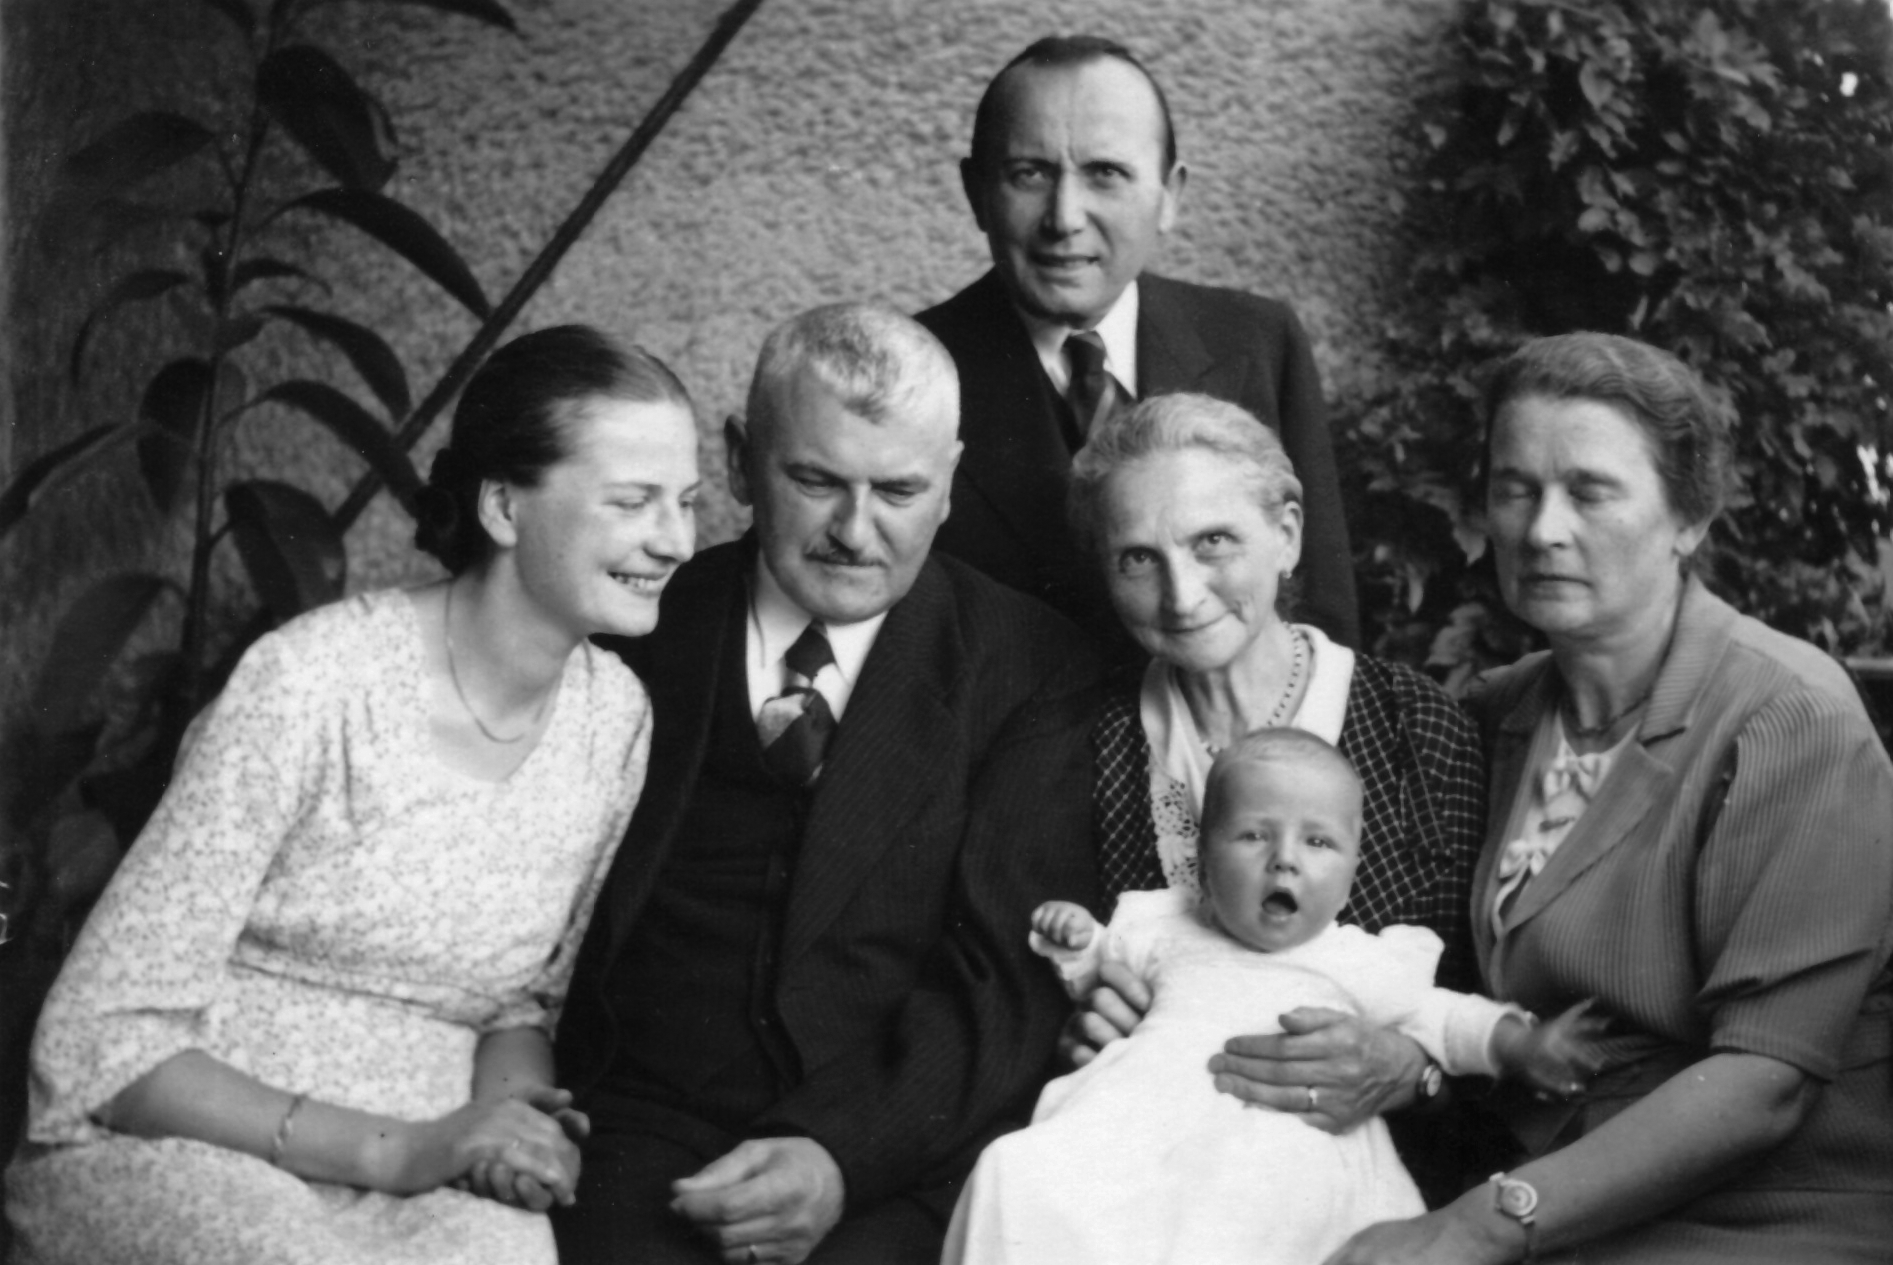
\includegraphics[width=\linewidth]{Photos/Wolfgangs_Taufe.png}}
	\caption[Wolfgangs Taufe]{Wolfgangs Taufe am 29. August 1937, von links nach rechts: Margot Busse, Otto Wernicke, Marie Mempel, Tante Friedel Wernicke, stehend: Emil Fache.\footnotemark}
	\label{fig:wolfgangs_taufe}
\end{figure}

\footnotetext{Anm. Helga: \enquote{Tante} Friedel war eine Cousine von Margot. Ihr Mann Otto war in Schlesien Landarzt. Genau wie wir flüchteten beide nach dem Krieg nach Magdeburg und wohnten nur wenige Minuten zu Fuß von uns entfernt. Nach der blutigen Niederschlagung des Aufstandes vom 17. Juni 1953 behandelte Otto nach Einbruch der Dunkelheit bei sich zuhause Leute, die in den Auseinandersetzungen verwundet worden waren.}

Mir war inzwischen am 1.4.38 die Leitung eines Bezirksseminars für die pädagogische Ausbildung der Studienreferendare übertragen worden. Ich verblieb mit 6 Wochenstunden am Elisabethgymnasium, hatte dort mein Amtszimmer und hielt auch dort meine Lehrsitzungen ab. Die Leitung des Elisabethgymnasiums war dem 150\%-igen Nazi und sturen Rassenfanatiker Dr. Fuchs übertragen worden, für den die Schüler schon nach 14 Tagen den treffenden Spitznamen \enquote{Polarfuchs} erfanden -- nordischer war nicht möglich! Mit diesem Herrn, der von sich sagte, seine Tragik bestehe darin, dass in ihm eine nordische Seele an einen ostischen Körper gebunden sei, hatte ich bald einige dienstliche Zusammenstöße, die den Stoff zu einer rassischen Groteske liefern können.

Das neue Amt nahm meine ganze Kraft in Anspruch, zumal ich u.a. wöchentlich eine 2-stündige Vorlesung über die Geschichte der Pädagogik mit besonderer Betonung der Probleme der Oberschule zu halten hatte. Die Prüfungen der Referendare fanden am Ende des 2. Ausbildungsjahres zentral vor einer Berliner Kommission statt; ich hatte die Genugtuung, dass meine eingehenden Berichte über jeden einzelnen Referendar und seine Prüfungsleistungen in Berlin ein günstiges Echo fanden.

Mit der oben genannten Hybris von Prag begann die Peripetie der nationalistischen und deutschen Tragödie. Der heiße Krieg mit den Westmächten stand vor der Tür.\marginpar{21} Und doch schien der atemberaubende Coup des Hitler-Stalin-Paktes vom 23. August 1939 den Optimisten, zu denen auch ich in den letzten Augusttagen '39 gehörte, ein retardierendes, vielleicht ein happyend ermöglichendes Moment zu sein -- war der sofort einsetzende Aufmarsch an der polnischen Grenze, dessen Augenzeuge jeder Breslauer wurde, nur ein Theatercoup?

Im Morgengrauen des 31. August donnerten Hunderte von deutschen Bombern, die Breslau in östlicher Richtung überflogen, ihr schreckliches Nein! herab. Das war der Weltkrieg: England und Frankreich, Polens Verbündete, erklärten uns den Krieg. Frankreich sprengte die Straßburger Rheinbrücke, in Breslau gingen abends \marginpar{22} die Lichter aus, englische Bomber begannen ihre Einflüge ins Reichsgebiet. Ich schachtete in unserem Garten -- wir hatten im Frühjahr 1939 ein Zweifamilienhaus mit großem Garten in der Mörikestraße gekauft und bezogen -- einen splittersicheren Unterstand aus.

Während unsere beiden kleinen Jungs von der Oma betreut wurden, verlebte ich um die Jahreswende mit Margot eine Skiwoche im Altvatergebiet des neuerworbenen Sudetengaues.

Nachdem meine Referendare ihre Prüfung abgelegt hatten, wurden sie, wie schon die meisten Referendare des 1. Jahrgangs zum Wehrdienst eingezogen, während die nicht einberufene Minderheit zu einem Seminar unter Direktor Jenthe zusammengelegt wurden. Ich trat zunächst in den Schuldienst am Elisabethgymnasium zurück, erlebte mit zwei Primen im Landheim im Juni 1940 jubelnd die Einnahme von Paris \marginpar{23} und den Waffenstillstand mit Frankreich im Glauben, dass Hitler nunmehr zu einem maßvollen Friedensschluss bereit sein werde.

Unmittelbar nach meiner Rückkehr aus dem Landheim erreichte mich meine Berufung ins Oberpräsidium Abt. Höheres Schulwesen, als \enquote{wissenschaftlicher Hilfsarbeiter} -- erfahrungsgemäß eine Übergangsstelle zu leidendem Posten. Mir oblag die Bearbeitung der Studienreferendarsangelegenheiten mit zunächst begrenzter Zeichnungsberechtigung.

Noch im Juli erhielt die Abt. Höheres Schulwesen, Leiter Präsident Prof. Dr. Wernen, wegen meiner Berufung vom Minister einen Rüffel: mein Parteigutachten hätte abgewartet werden sollen, und dieses -- in der Anlage beigefügte -- sei \marginpar{24} unzureichend; es lautete: \enquote{\ac{pg} F. Busse hat einen einwandfreien Charakter, er lässt aber jeglichen Einsatzwillen für die Bewegung vermissen.} Vom Abteilungsleiter erhielt ich die Weisung den NS Gaupersonalamtsleiter Friedrich aufzusuchen und mich um eine Bereinigung der Angelegenheit zu bemühen. Friedrichs Macht war beträchtlich, er konnte damals schon aus eigener Machtvollkommenheit \marginpar{25} Beamte wie Wirtschaftsführer einschließlich Generaldirektoren ihres Amtes entheben. Bei ungeschicktem Verhalten war mir meine Entlassung aus dem Schuldienst sicher. Friedrichs Haltung mir gegenüber war nicht unfreundlich, er gedachte kurz unserer Begegnung in der Schule Mitte der 20er Jahre, ich sei wohl ein tüchtiger Lehrer gewesen aber eine \enquote{Intelligenzbestie} (damals ein schlimmes Schimpfwort aus dem Munde der NS Funktionäre zur Bezeichnung von kritisch und selbständig denkenden und daher dem Nationalsozialismus nicht bedingungslos ergebenen Menschen) und so hätte ich laut Aktennotiz eine für einen bewährten Offizier des 1. Weltkrieges geradezu unglaubliche Äußerung getan -- ?? -- nämlich \enquote{Sie sollen nach der Einnahme von Paris \marginpar{26} geäußert haben: Wenn Hitler klug ist (unserer genialer Führer!!!) so schließt er jetzt einen Verständigungsfrieden}, \enquote{Eine solche anmaßende wahnsinnige Äußerung können Sie als Offizier doch gar nicht getan haben, das kann ich mir nicht denken!!} Jetzt log ich, musste ich lügen: \enquote{Nein, Gauamtsleiter, die habe ich auch nicht getan.}

Ich war gerettet; in strammer Haltung, Hacken zusammennehmend, wurde ich mit Handschlag verabschiedet.

\marginpar{27} Wie war die Bemerkung in meine Personalakten gekommen? Als einzigen Außenstehenden hatte ich sie zu meinem Haus- und Gartennachbarn Gasde gemacht, von Beruf Diplomingenieur, und da er Kapitänleutnant der Reserve, also Offizier war, glaubte ich an seinen anständigen Charakter. Wie ich erst nachträglich erfuhr, hatte er kurz vor unserem Gespräch am \enquote{Gartenzaun} das Amt eines Blockwarts übernommen und sich nun durch diese schamlose Denunziation bei der Partei Liebkind machen wollen.

Margot machte im August mit unseren beiden kleinen Jungs 14 Tage Ferien im Riesengebirge, ich musste zunächst auf Ausspannung verzichten.

Während Parteiversammlungen und auch Volksversammlungen mit dem Kampfgesängen endigend auf \enquote{Führer befiel! Wir folgen dir} und \enquote{Bomben, Bomben auf Engelland} schlossen, \marginpar{30} lief der für uns verlustreiche und das England Churchills nicht in die Knie zwingende Luftkrieg an. \marginpar{28} Im Spätherbst kursierten Gerüchte über nicht zu erfüllende Forderungen, die Molotow bei seinem Berliner Besuch gestellt habe.

Im Februar '41 ein missglückter Schiurlaub auf der Bradlerbaude mit Margot: mit Grippe fuhr ich hinauf, das Fieber stieg, Schwitzen nützte nichts, ich habe das Bett nicht verlassen können und wir fuhren nach 8 Tagen im Hörnerschlitten zu Tale.

Eine eingehende Untersuchung in der Klinik der Universität erwies, dass es eine hartnäckige Grippe war; sie wurde mit 2 Aspirintabletten geheilt.

Im Frühjahr bedrückten jeden urteilsfähigen Deutschen Gerüchte über den deutschen Aufmarsch an der deutsch-russischen quer durch Polen verlaufenden Demarkationslinie.

Margot fuhr mit den beiden Jungen in der 2. Maihälfte in das hinterpommerische Ostseebad Henkenhagen, ich folgte Anfang Juni als dort, wesentlich später als in Schlesien, \marginpar{29}noch die Obstbäume blühten und das Wasser der Ostsee mit nur 11° noch nicht zum Baden einlud. Wir wohnten hoch oben auf einer Düne in einem Fischerhause in einem schönen für Badegäste hergerichteten Südzimmer mit geschlossener Veranda. Zum breiten weichsandigen Strande führte eine Treppe hinab, ein herrlicher Tummelplatz für die Jungen, für uns alle recht erholsam, zumal die frischfischreiche Nahrung uns den Krieg fast vergessen ließ. Bedauernd packten wir am 21. Juni die Koffer zur Heimfahrt. Da weckte uns der Fischer Steinkraus um 5 Uhr morgens mit der atemberaubenden Radionachricht: \enquote{die deutschen Armeen sind auf breiter Front in die Sowjetunion einmarschiert.} Eine zutiefst bedrückende Meldung. Auf der \marginpar{30} ganzen Heimfahrt von Henkenhagen bis Breslau überall dumpfe Betroffenheit, kein fröhliches Gesicht.

Es folgten spannende Wochen: der besonders an der Nordfront sehr zähe russische Widerstand wurde überall langsam gebrochen, der Blitzangriff auf Moskau allerdings misslang. Einberufungen zur Wehrmacht. \ac{ostd} Fuchs (der \enquote{Polarfuchs}) verkündigte dem Kollegium des Elisabethgymnasiums in höchster Erregung: \enquote{Meine Herren! Mich, der ich gerade damit beschäftigt bin, das Waffenarsenal unseres Volkes von der sprachlich-rassischen Seite her zu stärken, mich zieht man zum Heeresdienst ein!!!} -- Allgemeines Schweigen. Eine Stimme, die des Physikers: \enquote{Tja, Herr Direktor, der nordische Mensch gehört an die Front!}

\marginpar{31} Der Vormarsch der deutschen Heere gen Osten schien unaufhaltsam, Leningrad wurde eingeschlossen, Weißrussland und die wichtigsten Städte der Ukraine wurden das Opfer siegreicher Kesselschlachten. \enquote{Polarfuchs} schrieb dem Kollegium (nach dem Muster Wilhelms II. von 1914): \enquote{Noch ehe das Laub von den Bäumen gefallen ist, werden wir in der Heimat sein.} Aber er hat sie, wie Millionen deutscher Soldaten, nicht wiedergesehen. Das Deutsche Oberkommando verkündete das siegreiche Ende des Russlandfeldzuges, und mit Pearl-Harbour traten USA und Japan in den Krieg ein. Und dem deutschen Soldaten stand ein harter russischer Winter bevor, mit dem man nicht gerechnet hatte. Die Bevölkerung wurde zur Abgabe von Pelzsachen und Skiern aufgerufen, auch wir trennten uns von Pelzsachen und von unseren Brettern.

\marginpar{32} Im Februar 1942, wo ich mit Margot 14 Tage Urlaub im \enquote{Wiesenhaus} von Oberschreiberhau nahm, verfolgten wir am Radio den raschen Siegeszug der Japaner in Ostasien auf Kosten von USA und vor allem Englands.

Im Frühjahr 1942, in dem wir am 8. Mai unser erstes Töchterchen Helga bekamen, ging der Bewegungskrieg in Russland mit großen deutschen Erfolgen weiter, doch in den westlichen Großstädten begannen angelsächsische Bomber bei nächtlichen Angriffen schmerzliche Verwüstungen anzurichten. Von den Vorgängen an der Ostfront und im besetzten Gebiet erfuhr ich dann und wann von beurlaubten Referendaren, die meist zu Offizieren aufgerückt waren, Dinge, die in den Wehrmachtsberichten und in der Presse verschwiegen wurden. Ich hatte noch eine andere Informationsquelle: die Kriegsteilnehmer, die zu Kursen zwecks Ablegung der Reifeprüfungen für \marginpar{33} mehrere Monate nach Breslau beurlaubt wurden. Ich leitete die Kurse und unterrichtete selbst so einen von ihnen.

Am 8. Mai wurde uns unsere Tochter Helga geboren. Daher verlebte ich meine restlichen Urlaubstage ohne Margot mit dem inzwischen 5-jährigen Wolfgang im Oberschreiberhauer \enquote{Wiesenhaus}.

In der Schulaufsichtsbehörde erweiterte sich mein Aufgabenkreis, ich führte die Verhandlungen mit der \enquote{Hitlerjugend}, übernahm die Aufsicht einer Reihe von Nichtvollangestellter, die ich revidierte mit anschließender Lehrerkonferenz, ich hielt einige Vorträge in der Universität und im Glatzer Gebirge über die Berufsausbildung des Lehrernachwuchses der Oberschulen.

Im Herbst 1942 verdüsterte sich für uns der militärische Horizont: die Armee des Gen. Obersten Paulus war in Stalingrad eingeschlossen, alle Ersatzversuche schlugen fehl; ich bekam zu hören, dass im Hauptquartier Hitler vor Wut die Nerven verloren habe, sich auf dem Boden wälzte und in die Teppiche biss. Mit der Kapitulation am 3.2.1943 schwand meine Hoffnung auf einen Sieg Deutschlands endgültig dahin.

\marginpar{34} Es begann der Rückzug auf breiter Front, der schließlich den Kampfeswillen der Truppe schwächen musste. Hitler ließ den \enquote{Totalen Krieg} verkünden, der jedoch -- im Gegensatz zur Sowjetunion -- meines Erachtens nicht wirklich durchgeführt wurde, z.B. wurden die Oberstufen der Oberschulen nicht, auch nicht einmal in den Ferien, zum Aufbau einer Verbindungslinie im Osten, z.B. am Dnepr, eingesetzt

\marginpar{35} Im Sommer 43 verbrachten wir zum letzten Mal unsere Ferien an der Ostsee in Henkenhagen. Margot war mit dem 6-jährigen Wolfgang und dem annähernd 5-jährigen Harald 14 Tage vor mir abgefahren, die Oma und unser Hausmädchen Inge versorgten mich. Meine Fahrt ging über Posen, ich sah die hohläugigen, abgemagerten Gesichter der wie Kriegsgefangene behandelten polnischen Bewohner unserer Provinz Posen\dots Ich wurde vom etwas landeinwärts gelegenen Bahnhof Henkenhagen mit einer Droschke abgeholt, den beiden Jungen waren Pferd und Wagen interessanter als der \enquote{Vati}, sie saßen auf dem Bock. Die Jungen sausten schon früh im Nachthemd die Treppe von Steinkraus' Haus zum Strande hinab, sie hatten Spielkameraden und -innen gefunden, das Wasser war hinreichend warm. Es war spaßig \marginpar{36} welche Tricks man jetzt anwenden musste, um seinen Bedarf an Fischen zu decken. Wir machten erholsame Dünenwanderungen, einige lustige Droschkenfahrten in die nähere Umgebung, einen Ausflug nach Kolberg -- doch unverkennbar, die Stimmung der Erwachsenen war gedrückt, von Fronturlaubern -- Offizieren -- vernahm ich nichts, dass noch irgend Hoffnung auf einen guten Ausgang hätte wachhalten können.

Auf einem Abschiedsabend meiner Kriegsabiturienten hatte der junge Westphale Dringenberg das Bedürfnis, sich von einer seelischen Last zu befreien oder wenigstens durch Mitteilung ihren Druck zu verringern. Was zutage kam war so entsetzlich, so schaurig, dass ich mehrere Nächte keinen Schlaf fand. Der 19-jährige Junge war von der Truppe in ein \enquote{Vernichtungslager} abkommandiert worden. Seine Gruppe, die ein Maschinengewehr zu bedienen hatte, wurde morgens um halb 6 Uhr geweckt. Jeder bekam auf nüchternen Magen 0,5 l starken Alkohol eingeflößt. Darauf sah man die Welt wie durch einen Schleier. \marginpar{37} Die Mannschaft wurde zu ihrem MG-Stand geführt. Das MG war auf eine breite Bohle gerichtet, die über eine riesige Grube gelegt war. Auf diese Bohle wurden nackte Juden getrieben, Frauen, Kinder, Männer, Greise und mit dem MG niedergeschossen. Sie stürzten schreiend und röchelnd, tot oder schwer verwundet nach beiden Seiten in das Massengrab. Dann betrat ein Mann mit einem Kasten die Bohle und streute ungelöschten Kalk auf die Niedergestürzten\dots Das Geschrei der oft nur verwundeten Unglücklichen war fürchterlich. Jeden Tag musste die Mannschaft auf diese Weise \num{3600} Juden \enquote{liquidieren}.

Dringenberg hat es nur 5 Tage ausgehalten, dann brach er seelisch zusammen und kam in eine Nervenheilanstalt. Nach 10 Monaten wurde er als gesund zur Front entlassen.

\marginpar{38} Sein Truppenteil stand einer Formation jüdischer Mädchen Soldatinnen gegenüber. Bei einem nächtlichen Patrouillenunternehmen gelang es den Deutschen, in die gegnerische Stellung einzudringen und heil zurückzukehren, nachdem sie einige jüdische Mädchen vergewaltigt hatten. Beim nächsten Patrouillenunternehmen von Dringenbergs Einheit geriet die Gruppe in einen Hinterhalt der jüdischen Soldatinnen, wurde gefesselt, man schnitt ihnen die Genitalien ab und ließ sie verbluten und verrecken.

Hass- und Rachegefühle loderten nun auf deutscher Seite jäh auf, \enquote{auch ich}, sagte Dringenberg, \enquote{wurde jetzt wieder ganz Soldat, der in einem unerbittlichen Kampf mit einem hasserfüllten und gnadenlosen Feinde steht}. Er jagte mit dem Rächertrupp vor und die Judenmädchen wurden nackt mit den Füßen an Baumästen aufgehängt; wollten sie sich in ihrer Qual aufrichten, hieb man mit Peitschen auf sie ein.

\marginpar{39} Für mich stand fest, dass der Krieg in Deutschland hoffnungslos verloren war und unsere Gegner sich böse an uns rächen würden. Dass wir fast ganz Schlesien verlieren würden mit Zustimmung der drei Westmächte und unter Nichtachtung einer 800-jährigen geschichtlichen Entwicklung -- das freilich hatte ich damals nicht für möglich gehalten. Mein persönlicher Leitgedanke war jetzt, sich nicht zu exponieren, alles das zu tun, war mir zum Überleben unserer Familie machbar erschien.

Im Herbst 43 fuhr Ob. Schulrat Diering mit mir nach Liegnitz zur Besichtigung der sogen. \enquote{Ritterakademie}, einer großen Anstalt mit Internat, die zu den \enquote{besonders bedeutsamen Oberschulen} Deutschlands zählte und dessen Direktor das Gehalt eines Oberschulrates erhielt. Ich beleuchtete den Schulbetrieb kritisch, machte eine Anzahl Verbesserungsvorschläge auf den verschiedensten Gebieten zur völligen Befriedigung Dierings, so dass er mir am Abend die Übernahme dieser Anstalt zum 1.4.44 antrug. Ich erbat mir eine Woche Bedenkzeit und erhielt zusätzlich die Genehmigung weiterhin in Breslau zu wohnen und täglich bei guter D-Zug Verbindung zum 70~km entfernten [Liegnitz] hinüberfahren zu können. Das Angebot \marginpar{40} war immerhin verlockend und hätte ich gewusst, dass ich dann heute eine weit höhere Pension bezöge, dann hätte ich vielleicht\dots, so war ich mir mit Margot rasch im Klaren: ablehnen, schon um nicht am Tage X auf offener Straße als evidenter Nazi totgeschlagen zu werden. Ich entsagte endgültig allen Ambitionen und beschäftigte mich wieder mit Russisch, das in Deutschland Seltenheitswert hatte und das meine und meiner Familie Überlebenschancen aufbessern könnte, eine Überlegung, die sich später als richtig erwies.

Dem Oberschulrat Dr. Etterich, dem meine Betroffenheit nach dem Abend mit Dringenberg auffiel, erzählte ich von dem Judenmassaker und fragte ihn, wie er sich verhalten würde, wenn an ihn das Ansinnen gerichtet würde, unschuldige Menschen niederzuknallen\dots seine Antwort war: \enquote{Wenn es der Befehl des Führers ist, würde ich ihn ausführen ohne mit der Wimper zu zucken.} Etterich belästigte mich von jetzt ab öfter mit Fragen wie: Herr B., sind sie überhaupt noch Nationalsozialist? Glauben Sie nicht mehr an die Genialität des Führers und unseren Endsieg?\footnote{Anm. Helga: im Alter von 14 Jahren besuchte ich im Sommer 1956 (also ein halbes Jahr nach der geglückten Flucht nach Westberlin) auf seine Einladung Dr. Walter Etterich in Hattingen. Sehr freundliche Aufnahme in der geräumigen Villa. Ich wurde an die Bücherwand geführt und sah eine für mich gewaltige Sammlung von und über Hitler. In Erinnerung sind mir \enquote{Adolf Hitler, mein Jungendfreund} und \enquote{Mein Kampf}. Ich hatte vorher noch nie von einem Buch gehört, was \enquote{Mein Kampf} hieß, und es hatte mich auch nicht interessiert. Herr Etterich war sehr überrascht und fragte mich: \enquote{Hat dir denn dein Vater nichts über unseren Führer erzählt?} Als ich verneinte, schien er unzufrieden. Meine Erziehung entsprach offensichtlich nicht seinen Vorstellungen.}\marginpar{41} Gefährliche Fragen in jeder Diktatur. Ich antwortete stets ausweichend, nämlich mit der Gegenfrage, was ihn denn zu dieser Frage veranlasse.

Übrigens war meine Hinwendung zum Russischen auch dem Umstand zu verdanken, dass ich seit 1941 neusprachlicher Berater des Schulbuchverlages Hirt in Breslau war und an einem russischen Lehrbuch mitarbeitete und zwar den phonetischen Teil schrieb. Ich erinnere mich eines interessanten \enquote{Arbeitsessens} im Hotel Monopol in Breslau Mai 1942 unter Vorsitz des Chefs des Hauses Hirt, der voll von Optimismus getragen war hinsichtlich des Russengeschäftes und im besonderen der Chancen seiner in Kiew gegründeten Niederlassung. Der Lesehunger, insbesondere die Nachfrage nach deutschen und westeuropäischen Büchern überstiege jedes erwartete Maß. Weniger als 2 Jahre später war mit der Räumung der Dnepr-Linie die schöne Seifenblase zerplatzt.

Im Jahre 44, an einem trüben Januartag mit so düsterem politisch-militäri\-schen Horizont wurde uns unser zweites Mädel Ulla geboren.

Unvergesslich ist mir das Kinderfest anlässlich Helgas 2. Geburtstag.

\section{Unternehmen Berthold}

Im Sommer des Jahres 1944 machte die Einschnürung Deutschlands mit der Landung der Angelsachsen in der Normandie, dem Vorrücken der Alliierten in Italien, der Landung der Alliierten an der Côte d'Azur und dem Vordringen der Russen bis in die Nähe der \marginpar{42} ostpreußischen Grenze rasche Fortschritte. Die Luftherrschaft über unser Land hatten wir längst eingebüßt, von Woche zu Woche wurden immer mehr deutsche Städte unter schrecklichen Menschenopfern von feindlichen Bombenflugzeugen verwüstet. Das missglückte Attentat auf Hitler blieb ohne Wirkung. Ende Juli erreichte mich in Bad Salzbrunn\footnote{Wohnort von Margots Mutter Marie Mempel}, wo ich mit der Familie kurze Sommerferien verlebte, das Telegramm von meiner Behörde sofort nach Breslau zurückzukehren. Jetzt endlich verwirklichte man den totalen Krieg auch in der Abt. Höheres Schulwesen -- allerdings viel zu spät, im Augenblick, wo uns das Wasser schon bis zum Halse stand: alles was irgend konnte, einschließlich der Oberschulräte an die Ostgrenze -- Schlesiens! um Panzergräben mit Hacke und Spaten auszuheben. Es wurde ein oben 3~m breiter Panzergraben ausgehoben, der etwa parallel zur deutsch-polnischen Grenze von 1919, also etwa einen von nordosten angreifenden Feind ausgerichtet -- oder verteidigte hier einfach der Gauleiter Schlesiens, Hanke, seine Provinzgrenzen? Die Gauleiter hatten sich ja inzwischen zu Gaukönigen herausgemausert. Die Ministerien in Berlin wagten nicht mehr in die Maßnahmen der Gaukönige einzugreifen. Da ich vom 1. Weltkriege her mein Interesse für militärische Strategie und Taktik wachgehalten hatte und mich arbeitsfähig fühlte, hielt ich die ganze Planung für falsch und meine Arbeit mithin sinnlos:

\marginpar{43}
\begin{enumerate}
	\item stellten so schmale Panzergräben für Angreifer wie die großen russischen bzw. amerikanischen Panzer kein ernsthaftes Hindernis dar
	\item würde ja wahrscheinlich der Russe über Oberschlesien, also von SO aus die Front aufrollen -- wie es dann auch im Januar 45 geschah
\end{enumerate}

Das Zentrum unseres Abschnittes des \enquote{Unternehmen Berthold} war Trachenberg, wo ich zunächst im Massenquartier einer Volksschule, dann mit ärztlicher Hilfe in Privatquartieren untergebracht war. Wir rückten täglich 4 Uhr morgens ab zu unserer etwa 4~km entfernten Arbeitsstätte, schanzten dort 8 Stunden und kehrten zum Mittagessen zwischen 1 und 2 Uhr heim. Mein Ziel war, mich bei dieser schweren, ungewohnten und, wie mir klar war, sinnlosen Schanzarbeit meine Gesundheit nicht durch Überanstrengung zu gefährden, wie es so manchem erging. Ein Hundertschaftführer meldete mich, dass ich im Zusammenhang mit Austreten sogar Schmetterlingsjagd betrieben habe. Ich wurde in Trachenberg bei \marginpar{44} einem Appell vom Tausendschaftsführer -- zwar ohne Namensnennung -- gerügt: \enquote{Die laxe Arbeitsmoral gehe bei manchen so weit, dass sie sich nicht scheuen, während der Arbeitszeit, wie z.B. ein Studienrat, Schmetterlinge zu fangen!!} Ich erhielt Befehl zum Austreten nicht in den Wald zu gehen, sondern nur die Bretterbude -- eine für 500! Mann -- zu benutzen, was ich jedoch aus hygienischen Gründen ablehnte, und ich habe mich durchgesetzt. Der Hundertschaftsführer wachte mit der Uhr in der Hand darüber, dass ich nicht zu lange fortblieb\dots Wenn ich Wochenendsurlaub erhielt, nahm ich Brote nach Breslau bzw. Salzbrunn mit: ich tauschte bei Berthold meine \enquote{Empfangszigaretten} gegen Brote, und zwar gab man mir für 3 Zigaretten 1 Brot; sie wurden von Margot und Inge in Schnitten zerteilt, getrocknet und dann zu Krümeln gerieben und in Säckchen gespeichert; auf diese Weise ergatterte ich auch mal etwas Zucker.

Eines Oktobersonnabendnachmittags hatte mich Margot in Trachenberg besucht und wir \marginpar{45} fuhren beide mit dem Eilzug nach Dresden, wohin auch die Kinder mit Oma aus Salzbrunn zur Walnussernte gekommen war. Vom Zug aus bemerkten wir plötzlich in der Luft -- es war schon dunkel und die Abteile nicht beleuchtet -- schräg über uns große, anscheinend feststehende Leuchtkörper. Unser Zug hielt in einem Waldstück, wir hörten, dass ein Bombenangriff auf Dresden im Gange sei. Wir hielten und hielten über eine Stunde; offenbar musste erst geprüft werden, ob der Bahnkörper während des Bombardements etwa beschädigt war. Schließlich fuhren wir im 30 km/h-Tempo weiter, konnten am Hauptbahnhof in Dresden aussteigen und zu Fuß nach Hause laufen, wo wir gegen Mitternacht eintrafen. Die durch 80 russ. Bomber bei geringer deutscher Flugabwehr hervorgerufenen Schäden waren nicht sehr groß. Dieses Ereignis war für unsere beiden Jungen höchst spannend gewesen, zumal eine Bombe \enquote{nur ein paar Minuten vor uns eingeschlagen waren und einen Brand verursacht hatte}. Der russ. Angriff war offenbar mehr auf psychol. Wirkung berechnet und hatte damit auch sein Ziel erreicht. Die Breslauer waren wegen der \marginpar{46} Schwäche und Erfolglosigkeit unserer Luftabwehr bedrückt.

Im November wurde ich für 14 Tage in die Abt. Höheres Schulwesen im Oberpräsidium zurückgerufen: Referendarangelegenheiten, Teilnahme an Assessorenprüfung, Korrekturen von Abiturientenaufsätzen mit mündlichen Prüfungen in Deutsch und Französisch. Den Vorsitz der Assessorenprüfung hatte ein Regierungsdirektor aus dem Berliner Kultusministerium. Unvergesslich ist mir seine Schilderung im kleinen Kreise von den Zuständen im zerstörten und brennenden Berlin, wie er selbst mit der im Handwagen geretteten Habe nachts stundenlang mühsam durch dampfende Trümmer vorbei an brennenden Häusern gezogen sei. Aber er schloss seine Ausführungen mit Gedanken wie: \enquote{Und wenn unsere Feinde all unsere Städte mit den großen Rüstungsschmieden zerstört haben, wir sind dabei in den Wäldern neue zu bauen und von den Wäldern aus erbarmungslos weiter zu kämpfen bis zum Endsieg.} Ich war verblüfft über diesen militärischen und rüstungstechnischen Unsinn -- oder schwatzte der Herr Ministerialdirigent nur so um nicht in \marginpar{47} den Verdacht eines verbrecherischen Defätismus zu geraten?

\marginpar{19.10.1976} Nach Beendigung meines \enquote{Diensturlaubs} fuhr ich nach Trachenberg zurück, fand meine \enquote{Barthold}-Abteilung nicht mehr vor: sie war jetzt 20~km östlich in Fürstenberg an der Kleinbahnstrecke nach Militsch, einer waldreichen Gegend. Ich sägte in einem Gruppenverbande täglich 8 Stunden mit einer einfachen Bogensäge Baumstämme, was meine Armmuskeln kräftigte. Der Tausendschaftführer war ein junger ehemaliger Elisabethaner, der mich kannte. Ihm unterstand auch ein Lager mit etwa 200 Franzosen, jüngere bis mittlere Jahrgänge, mit denen man große Schwierigkeiten hatte: faule Drückeberger, über die die Hundertschaftführer fast täglich sich beschwerten; \enquote{eine faule renitente gefährliche Bande, bei der auch Stockhiebe nichts ausrichten.}

Ich sollte das Amt des Dolmetschers und so etwas wie inoffiziellen Leiters des französischen Lagers übernehmen. Ich bat um Bedenkzeit, um mir erst einmal die Franzosen anzusehen und anzuhören. Ich bekam keinen schlechten Eindruck \marginpar{48}von den Franzosen, die zum großen Teil aus Paris und weiteren Umgebung stammten und fand ihre Beschwerden durchaus gerechtfertigt: sie wollten keinesfalls mit Italienern, wie man es ihnen zumutete, gemeinsam in der gleichen Baracke untergebracht werden, mit Angehörigen dieses gemeinen raubgierigen Volkes, von denen sie feige überfallen worden seien, in dem Augenblick, als Hitler Frankreich zu Boden geworfen hatte. \enquote{Zusammen mit diesem Pack -- nein, da würde es Mord und Totschlag geben}, so ihre Worte.

Als Bedingung für die Übernahme des Dolmetscher- und Berateramtes stellte ich dem Tausendschaftsführer die Forderung:

\begin{enumerate}
	\item keine Zusammenlegung mit Italienern
	\item keine, wie es bisher oft geschehen sei, Unterschlagung der den Franzosen zustehenden Zigarettenrationen und weitere Schmälerung ihrer Rechte
	\item den Hundertschaftsführern strengsten zu verbieten, die Franzosen zu schlagen
\end{enumerate}

Der Tausendschaftsführer stimmte mir restlos zu, hielt bei meiner Einführung als Dolmetscher und Berater eine Ansprache ganz in meinem Sinne, die ich Satz für Satz ins Französische \marginpar{49} übersetzte. Ich meinerseits hielt noch eine französische Ansprache, die dank meiner Kenntnisse der nationalfranzösischen Mentalität gut ankam.

Bei den Dienstbesprechungen mit den Hundertschaftsführern, zu denen ich jetzt herangezogen wurde, lobte man jetzt das Verhalten der Franzosen, sie hätten sich völlig gewandelt, arbeiteten fleißig, es gäbe keine Ärgernisse mehr mit ihnen. Meine Franzosen erwiesen sich übrigens als Lebenskünstler: ging ich zur Mittagszeit durch ihre Baracke, so bruzelte zusätzlich zum empfangenen Feldküchenessen hier ein Kaninchen, dort Fische oder gar ein Schweinebraten; auf meine Frage, wie sie das \enquote{organisiert} hätten, schwiegen sie verschmitzt lächelnd. Bei der Durchsicht ihrer Privatkorrespondenz, die zu meinem Aufgabenbereich gehörte, fiel mir auf, dass eine ganze Reihe mit Schreibmaschine geschrieben war. Kein Franzose besaß im Lager diese technische Errungenschaft ebenso wenig wie einer der zahlreichen Barthold abkommandierten \enquote{Akademiker}! Lösung des Rätsels: die charmanten Franzosen hatten es verstanden, sich die Gunst der Bürosekretärinnen zu erwerben\dots

\marginpar{50} Ein handgeschriebener Brief ist mir unvergesslich. Der Verfasser hatte mit einem deutschen Mädchen ein Kind, \enquote{sein} und \enquote{unser} Kurtchen, wie er in ziemlich gutem Deutsch schrieb. Der fast 3 Seiten lange Brief handelte von liebevoller Phantasie getragen ausschließlich davon, was und wie die junge Mutter mit dem geliebten Jungchen spielen würde. Die Mutter wird ihn mit Tränen der Rührung gelesen haben. Nur der Schluss enthielt eine erotische Anspielung: \enquote{Die Nächte hier sind kalt. Da sehne ich mich so nach die Hitze deines Körpers.}

Ich bekam den Auftrag, am 24.12. vor den 350 Lagerinsassen die Weihnachtsrede zu halten. Der Lagerleiter drohte, er werde genau aufpassen, dass ich kein Wort spreche, das der Lehre des Nationalsozialismus zuwider sei. Ich hielt also eine Art germanisch folkloristisch gefärbter Sonnwendfeier ab.

Zum Weihnachtsfest -- 2 Tage Urlaub -- brachte ich den Kindern einen Rucksack voll dicker Kiefernrinde mit, aus der ich mit ihnen Schiffchen schnitzte.

Um Neujahr regte der Lagerleiter an, es soll doch jemand allabendlich anhand einer Landkarte vor den Lagerinsassen einen natürlich von Siegeszuversicht getragenen Bericht über die militärische Lage halten. Mein Schlafgenosse, ein Breslauer Diplomingenieur meinte, das könnten wir beide doch gemeinsam übernehmen. Als ich ablehnte mit der Begründung, dass doch an Sieg gar nicht mehr zu denken sei und unser völliger Zusammenbruch doch nur noch eine Frage von Monaten sein könne, war er entsetzt und völlig niedergeschlagen. Er habe bis jetzt fest an unseren Endsieg geglaubt. Mein Zimmernachbar war wenigstens ein anständiger Charakter; ein Schuft wie Gasde hätte mich gemeldet und ich wäre, wie in den ersten Monaten '45 so viele, wegen Defätismus erschossen worden.

Etwa 3~km entfernt von uns befand sich ein Lager jüdischer Frauen, die an manchen Tagen in der Nähe unseres Lagers schwere Arbeit z.B. Tragen von Baumstämmen, zu verrichten hatten. Die Unglücklichen stürzten sich auf die Müllkübel und suchten nach Speiseresten, fingen dankbar Kartoffeln und Kartoffelstückchen auf, die ihnen von einzelnen Mitleidigen unseres Lagers zugeworfen wurden. Wurde eine von den \marginpar{52} unglücklichen Jüdinnen dabei erwischt, kriegten sie von den tierischen Henkersknechten, ihren \enquote{Wächtern}, Schläge mit groben Knüppeln. Jeden Abend, nach Einbruch der Dunkelheit, fuhr an unserem Lager vorbei ein Karren mit verreckten, verhungerten oder sonstwie zu Tode gebrachten oder mangels jeglicher ärztlicher Betreuung gestorbener Frauen.

Es kam der 12. Januar 45. Durchbruch überlegener russ. Streitkräfte auf breiter Front und Einkesselung großer deutscher Verbände. Bald sah man in dunkler Frostnacht im Osten fernes Aufblitzen weit außerhalb der Schallreichweite; wahrscheinlich Sprengungen von Brücken u.ä. durch die restlichen sich eilig zurückziehenden deutschen Truppenverbände.

Ich bekam einen Eilbrief von Ella, ich solle mich schleunigst nach Trachenberg zur Untersuchung durch den maßgeblichen Bartholdarzt begeben, der Bescheid wisse und mich krankschreiben werde, so dass ich noch mit der Bahn zu meiner Familie fahren könne. Ella, die treue Seele, hatte offenbar den Arzt mit Wein und Likör bestochen. Ich wurde krank geschrieben.

\marginpar{53} Die Franzosen hatten mir einen Schlitten zurechtgezimmert, auf dem ich auf vereister und verschneiter Straße mein Handgepäck transportieren konnte. Leider habe ich die Adressen der Guten, die sich von mir wie von einem Freund verabschiedeten, nicht aufgeschrieben. Sie hatten mich kurz zuvor noch um Rat gefragt, ob es im allgemeinen Wirrwarr des Zusammenbruches vielleicht für sie zweckmäßiger sei, zu den Russen zu laufen statt mit den Deutschen zu fliehen. Vor einem solchen Schritt warnte ich sie; bei einem stets möglichen kleinen erfolgreichen Gegenangriff der Deutschen würden sie als Überläufer an die Wand gestellt und erschossen. Sie sahen die Richtigkeit meines Rates sofort ein.

Am Nachmittag des 21. Januars rückte ich mit meinem Schlitten ab, 20~km bis Trachenberg. Die Kleinbahn Militsch-Trachenberg hatten den Verkehr bereits eingestellt. Unterwegs wurde ich überholt von einem langen Trupp abgezehrter jüdischer Frauen, die von bestialischen menschlichen Ungeheuern zur Eile mit Knüppeln angetrieben wurden. Wer zusammenbrach erhielt soviel Stockschläge auf den Rücken bis die Arme schreiend unter letzter Kraftanstrengung sich weiter schleppte. Für \underline{mein} Überleben war es ein Glück, dass ich waffenlos war, ich hätte mich schwerlich davon zurückhalten können, die abscheulichste dieser menschlichen Bestien niederzuschießen.

Nach langem Warten auf dem Bahnhof Trachenberg kam, wie es hieß, der letzte Zug aus dem Posenschen an. Er war endlos lang, schrecklich überfüllt mit Flüchtlingen. Ich erhielt einen Sitzplatz. Der Zug fuhr ganz langsam ohne zu halten und kam erst bei Tagesanbruch auf dem Breslauer Hauptbahnhof an. Ich begab mich sofort in das Bürohaus von Faches in der Gärtnerstraße gegenüber dem Hauptbahnhof, wo ich schon Ella und Emil [antraf]. Wir besprachen die Lage: Breslau werde in Kurzem eingeschlossen sein und sich als Festung verteidigen. Emilio hatte sich, entgegen früheren Absichtsäußerungen, entschlossen in Breslau zu bleiben. Ich war betroffen, um nicht zu sagen entsetzt. Sie wollten ihr Haus am Stadtrande aufgeben und sich in die innere Stadt zurückziehen. Dass ich zu meiner Familie \marginpar{55}nach Bad Salzbrunn gehe, hielten sie für selbstverständlich. Mit Tränen in den Augen nahm ich von ihnen Abschied. Ellas letzte Worte waren: es wird schon alles gut ausgehen. Ich sollte sie jedoch nie wieder sehen.

In Breslau herrschte ein riesiges Kommen und Gehen, nein, richtiges Laufen und Hasten. Alles war im Aufbruch. Ich sammelte in unserer Wohnung noch einige Habseligkeiten s.a. Familienbilder und verstaute sie im Koffer und schleppte mich zum Freiburger Bahnhof, denn die Straßenbahn verkehrte nicht mehr. Im Radio war durchgegeben, dass das rechte Oderufer aufgegeben werde.

Auf der Strecke Breslau-Waldenburg verkehrten viele außerplanmäßige Züge in annäherndem Personenzugtempo. In Salzbrunn lag Schnee, ich rodelte mit den Kindern. Ich dachte nicht daran zum Arzt zu gehen, hatte ich doch einen Krankenschein in der Hand und kümmerte mich zunächst auch nicht um den Standort von Barthold, dem ich ja noch angehörte. Noch war Breslau nicht von den Russen eingeschlossen, und so benutzte ich am 6. Februar, gegen Margots Willen, eine Autobusgelegenheit nach Breslau, \marginpar{56} um aus unserer Wohnung noch Kleidungsstücke u. anderes zu holen. Die Bahnunterführung zwischen Kleinburg und dem Breslauer Südparkviertel war vom deutschen Militär -- Landsturm -- gesperrt, es hieß alles aussteigen, der Zugang nach Breslau ist überall gesperrt. Ich ging mit meinem leeren Koffer die etwa 3~km bis zur Bahnunterführung, durch die man in Kürze in die Sauerbrunnsiedlung und somit in unser Haus, unweit des Bahnkörpers der Umgehungsbahn gelangen konnte. Doch der Durchgang war dicht verbarrikadiert, nur durch ein \enquote{Fuchsloch} konnte man in gebückter Haltung hindurch und dieses Fuchsloch war durch ältere Hitlerjungen versperrt. Es gelang mir, den leitenden Jungen zu überreden mich ausnahmsweise, da ich in unmittelbarer Nähe wohnte, durchzulassen. Unsere Wohnung war von Landstürmern besetzt, die sehr erschraken, als ich mich als Hausbesitzer und Wohnungsinhaber entpuppte. Der Grund des Schocks: es waren schon allerhand Gegenstände verschwunden, außer den Lebensmitteln und dem Weinvorrat im Keller fehlten Wolldecken, Schuhe und vieles andere, u.a. das schöne Ölbild, das Freund Bantau in meinem Auftrag angefertigt hatte: Hintergrund die noch schneebedeckten Bergrücken des Riesengebirges, in Vordergrund die Vorberge, in denen der Frühling schon seinen \marginpar{57} Einzug gehalten hatte. Mit den schönen Möbeln des Ess- und Kinderzimmers hatte man die nach SW gehenden Fenster fest verbarrikadiert, vom Balkon führte ein Laufgraben zum Luftschutzgraben, den ich schon 1939 bei Kriegsausbruch angelegt hatte. Ich versammelte den Zug und seinen Führer, einen Vizefeldwebel, in meinem Arbeitszimmer und belehrte sie anhand des Diercke-Atlasses, dass Breslau zu Deutschland gehört\dots Sie verstanden mich, aber was half es?

Es begann schon zu dämmern und ich machte mich mit meinem prallen Koffer auf in der Hoffnung, von der Ausfallstraße am Südpark mit einem Omnibus die Rückfahrt anzutreten und vielleicht vorher noch zu Faches Haus zu gehen. Dieser Illusion wurde ich schon nach 5 Minuten Weges jäh beraubt durch einen Landsturmmann: \enquote{Wohin wollen Sie? Heraus aus Breslau? Völlig ausgeschlossen, alles ist gesperrt, höchste Alarmbereitschaft, Russen sind bei Steinau über die Oder vorgedrungen, werden in wenigen Stunden vor Breslau sein. Also zurück!}

\marginpar{58} Zögernd machte ich kehrt, meine Lage überdenkend: ich werde also in den Landsturm eingereiht werden mit der aussichtslosen Aufgabe Breslau zu verteidigen. Werde ich meine Familie wiedersehen? Schwerlich. In diesen Gedanken störte [mich] an der Ecke Lenaustraße, 150~m von meinem Haus entfernt, ein großer Lieferwagen, dessen Fahrer mich nach der Ausfallstraße nach Schweidnitz fragte. Er habe sich verfahren. Ich sagte ihm, dass die nach Westen führenden Bahnunterführungen völlig verbarrikadiert seien. Während ich dies sagte, entdeckte ich die Firmenaufschrift auf dem Wagen Emil Fache AG. Der Fahrer kannte meinen Namen als Schwager Faches und verstaute mich in seinem vor allem mit Matratzen vollgestopften Fahrzeug, das jedoch in der Mitte einen Hohlraum von vielleicht 1,5 qm Bodenfläche besaß, in dem 2 Facheangestellte standen zu denen ich nun als Dritter kam. Der Wagen sauste zurück zur Südparkunterführung; dort hieß es halt! Strenge Prüfung des Inhalts, herzklopfend hörten wir Fragen und Antworten -- das Glück war mit uns: die Durchsuchung gelangte \marginpar{59} nicht bis zu unserem Versteck. In der Nacht erfolgten noch vier weitere Überprüfungen, wiederum Herzklopfen mit angehaltenem und schließlich mit befreitem Ausatmen. An einem Bahnhof einer noch in Betrieb befindlichen Bahnstrecke wurde ich abgesetzt, wartete stundenlang auf den nächsten Zug und landete im Morgengrauen in Waldenburg. Ich war gerettet. Zufall? Schicksal? Fügung? Gibt es Schutzengel? Nun, die Wahrscheinlichkeit meines Zusammentreffens mit dem Wagen meines Schwagers, der sich verfahren hatte um ca. 2~km und mir gerade in der Sekunde begegnete, als ich die Ecke Lenaustraße, ohne auch nur einen Funken Rettung zu sehen, erreichte, war nicht größer als meine Chance im Lotto mit 6 richtigen Zahlen zu gewinnen.

Um die Mitte Februar fuhr ich auf einem Lastwagen über Schweidnitz nach Reichenbach; wie auch schon in Salzbrunn vernahm man auf der ganzen Strecke deutlich den Kanonendonner, die Russen waren bis etwa Striegau, Janer, Zobten vorgedrungen. Meine Barthold-Abteilung baute in Peterswaldau Straßenschanzen und war im Saale des ersten \marginpar{60} großen Gasthofes in Steinkunzendorf untergebracht und ich schloss mich einer kleinen wie Kletten aneinanderhängenden Gruppe von Geometern an. Man hatte großspurig verkündet \enquote{die Sudeten würden in ein riesiges Verhau verwandelt, an dem die rote Flut zerschellen werde.} Sancta Semplicitas! Auch eine Abteilung jüngerer jüdischer Männer wurde in unserer Nähe unter SS-Aufsicht beschäftigt. Sie trugen alle schwarze, der HJ ähnlich geschnittene Kleidung, auf dem Rücken ein riesiges mit Ölfarbe gepinseltes Kreuz der Westkirche. Ich fragte einen SS-Scharführer, was das zu bedeuten habe. \enquote{Das Kreuz ist das Zeichen der Schmach; wenn wir mit den Juden fertig sind, kommen die Katholiken an die Reihe!} Eine französische Gruppe arbeitete neben uns; sie sagten mir: \enquote{Welch ein Unsinn, unsere Arbeit, es ist doch klar, dass Deutschland die Partie verloren hat, es sollte doch Schluss machen.} Ich erblickte eine Schwadron, die aus den Bergen zu Tale Richtung Front ritt: es waren russische, wohl meist ukrainische Kavalleristen, die unter Führung von General Wlassow auf unserer Seite gegen die Bolschewiki kämpften, sie wurden von russischen Kriegsgefangenen, die in Zivil auf \marginpar{61} deutschen Bauernhöfen arbeiteten, laut verhöhnt. Nicht wenige von diesen russischen Kriegsgefangenen ersetzten den im Felde stehenden Mann sowohl in der Wirtschaft wie im Schlafzimmer.

Die Russen beherrschten offenbar den ganzen schlesischen Luftraum schon im Februar: ich habe kein einziges deutsches Flugzeug am Himmel gesehen; ein einziger deutscher Helikopter, der über Peterswaldau einen Erkundigungsflug zur Front machen wollte, war im Nu von zwei russischen Jägern eingekreist und abgeschossen. Wir sahen und vernahmen den Sturz und den Aufschlag auf die Erde ca. 1~km von uns entfernt.

Nach knapp 3 Wochen erwirkte ich Wochenendurlaub zum Besuch meiner Familie in Salzbrunn, obwohl ich bei der Barthold-Leitung übel angeschrieben war und meine Personalakte, wie ich zu hören bekam, einem Saustall glich (von \enquote{Schmetterlingsjäger}, zu geringe Schanzleistung, Weigerung das Massenscheißbüdchen zu benutzen, Weigerung 1 Zentner schwere Säcke abzuladen, Entfernung von der Arbeitsstätte etc.)
Ich brach im Morgengrauen zu Fuß durchs Entengebirge auf, machte Frühstückspause mit einer durch die russische Front geflohenen Bäuerin, die mir erzählte: Nein! Was sind die Russen doch für komische Menschen; da sagen sie, das hier (sie deutete auf ihr Stück Brot) ist Klep! Wo \marginpar{62} das doch Brot ist, Brot! und da sagen sie: njet, das ist Klep!!

Da ich noch gerade eine Straßenbahn im äußersten Vorort von Waldenburg erwischte, langte ich um 13 Uhr in Salzbrunn an -- und fand das Nest verlassen vor: meine Familie war, wie alle Familien mit mehreren Kindern, evakuiert worden, und ich hörte von den Nachbarsleuten Trompka, bei denen ich mehrere Stunden blieb, dass sie nach Treuenbrietzen zu Margots Verwandten gefahren seien. Der Kanonendonner kam schon aus der Nähe, die Russen standen bei Freiburg. Dass sie nicht Salzbrunn und Waldenburg bombardierten war offenbar dem Umstand zu verdanken, da sie wussten, dass das Waldenburger Industriegebiet und ganz Schlesien ihnen als reife Frucht in den Schoß fallen werde. Mich betrübte weniger die Flucht meiner Familie an sich, als vielmehr das Fluchtziel Treuenbrietzen in der Nähe Berlins, wo, wie ich fest glaubte, die letzten schweren Kämpfe mit den Russen stattfinden würden. Noch in der ersten Märzdekade rückte Barthold weiter nach Westen auf Waldenburg zu in eines der langgestreckten Gebirgsstraßendörfer. Wir fällten herrliche Lärchen zum Bau von Straßensperren aber auch für Unterstände für Geschütze und in Schützengräben. Hier hatten wir als Arbeitsnachbarn Ukrainerinnen und Ukrainer, nach Kompanien gegliedert.

\marginpar{Ende \enquote{Meine Lebenserinnerungen im Abriss} Heft 1 bis März 45}

\marginpar{Abschrift beendet 7.5.2021}

\marginpar{\enquote{Meine Lebenserinnerungen im Abriss}, Heft 2 ab März 1945 -- verfasst im Diakoniekrankenhaus ab Anfang Okt. 1976}

\marginpar{63} Wir waren in Bauernhäusern untergebracht, von denen manche schon durch Zwangsevakuierung oder durch eigenwillige Flucht leer standen. Die Ukrainer, die meist schon seit 1942 oder '43 zur Arbeit nach Deutschland verschleppt waren, waren meist sympathische Leute, die das von ihnen Verlangte fleißig taten, und die, da sie meist schon etwas Deutsch gelernt hatten, bei Gelegenheit mit den Deutschen plauderten und selbst sich neckten. Die Mädchen erzählten mir u.a. durch den Kommunismus sei auf dem Lande der Gegensatz zwischen arm und reich größer geworden als früher, da die Funktionäre und Parteikommunisten für die fast gleiche Arbeit ein Vielfaches an Lohn bekämen. Für die Heiratsaussichten der Mädchen spielen Aussteuer und Mitgift im kommunistischen Staat eine große Rolle. In den Arbeitskompanien gab es auch einzelne ukrainische Ehepaare. Von einem solchen wurde ich zur abendlichen Sauerampfer-Kartoffelsuppe eingeladen, die mir trefflich mundete. Unweit meiner Arbeitsstätte befand sich ein Bauernhof, der von einem ukrainischen Kriegsgefangenen betreut wurde, einem \marginpar{64} jungen intelligenten und sehr gut aussehendem Manne, zu dem man Zutrauen haben konnte. In diesem Bauernhause machte ich öfters Frühstückspause; wechselte Michail, so hieß er, seine Kleidung, so tat er dies mit größter Selbstverständlichkeit im Schlafzimmer der Bäuerin, die mir, befragt, etwas verschämt erzählte, ein wie fleißiger, wie tüchtiger, guter und lieber Mensch dieser Michail sei. Durch ihn lernte ich durch Zufall Krimtšuk (\textcyr{Крымчук}), Professor der Geographie aus Melitopol kennen, der als Dienstverpflichteter 1943 nach Deutschland kam und von der Leitung des Unternehmens \enquote{Berthold} als Zeichner verwendet wurde. Aber sein Name war bis zur Universität gedrungen, und so hatte man ihn für kurze Zeit nach Dresden beurlaubt, wo er einen fachwissenschaftlichen Vortrag in der Universität hielt. Er war glücklich in mir einen gebildeten Menschen gefunden zu haben, mit dem er sich in seiner Muttersprache über die ernsthaftesten Dinge unterhalten konnte; seine Schulkenntnisse in westlichen Sprachen waren dürftig. Oft, wenn ich müde von der Arbeit kam, saß er schon auf meinem Bett und wartete auf mich. Er ließ mich geduldig essen und eine Stunde schlafen um dann mit mir offen über alles Erdenkliche zu sprechen. Seine Familie hatte ein schreckliches Schicksal erlitten. Sein \marginpar{65} Frau und seine drei Töchter erhielten Befehl, mit den zurückweichenden Deutschen, wie die andere ukrainische Zivilbevölkerung, Haus und Hof zu verlassen. Als sie sich weigerten, ihr schönes Haus mit den 8 Zimmern -- der geistigen wissenschaftlichen Elite machten die Bolschewiki Komfortzugeständnisse -- wurden alle vier kurzerhand von SS-Leuten erschossen. Und trotzdem blieb er als Nationalukrainer Feind der Bolschewisten. Er hoffte, dass die Amerikaner von der Elblinie ausgehend die völlig erschöpften sowjetischen Heere zurückschlagen und Europa einschließlich der Ukraine vor dem Bolschewismus retten würde -- täten sie es nicht, so wäre das eine solche Wahnsinnstat, wie man sie den Amerikanern doch nicht zutrauen könne. Krymtschuk hatte, wie er mir erzählte mehrfach in Versammlungen seine ukrainischen Landsleute zum Widerstand gegen die Bolschewiki und zur Unterstützung Wlassows aufgerufen.

Die Bertholdleitung hatte irgendwie herausbekommen, dass ich Offizier des 1. Weltkrieges war, und so ließen sie mich ohne mich überhaupt zu fragen, am Panzerabwehrgeschütz, der \enquote{Panzerfaust} ausbilden: ich sollte an der Spitze eines Trupps die vordringenden Russen zurückschlagen oder wenigstens aufhalten -- ein sinnloses, absolut aussichtsloses Unterfangen, das nur mit dem Blutopfer unserer Gruppe enden konnte. Zu meinem Trupp gehörte ein Breslauer Amtmann namens Schulz und ein \marginpar{66} elsässischer Gerichtsassessor aus Straßburg, die meine Vertrauten waren. Ihnen offenbarte ich, dass ich den angekündigten Wahnsinnsbefehl keinesfalls ausführen, sondern notfalls den, der mir einen solchen Befehl erteilen, niederschießen würde. Beide pflichteten mir bei. Meine praktische Ausbildung an der Panzerfaust musste zwar alsbald unterbrochen werden, da beim Übungsschießen, wie sich herausstellte, durch den starken Knall die eustachische Röhre meines rechten Ohres eingedrückt war, ich auf dem rechten Ohr nichts mehr hörte und ich wöchentlich 2x zum Ohrenarzt nach Waldenburg geschickt werden musste. Das änderte jedoch nichts an der mir für den Tag X übertragenen militärischen Fraktion.

Die Hoffnung, vielleicht über Trompkas ein Lebenszeichen von meiner Familie zu erhalten, trieb mich immer wieder an den Wochenenden nach Salzbrunn. Einmal langte ich dort erst völlig durchnässt gegen Mitternacht an, ich war in ein schweres, regenreiches Gewitter geraten. In Omas Bodenkammer lagerte das getrocknete Brot in Säcken, desgleichen etwas Zucker und einige Töpfe mit eingekochten Stachelbeeren: eine willkommene Aufbesserung meiner kargen Verpflegung. Kam ich an Feldern vorbei, \marginpar{67} suchte ich Sauerampfer, den ich seit meiner Kindheit gern mochte und pflückte wenig mundenen Klee\dots um meinen Magen mit den vielleicht bevorstehenden schlimmen Ernährungseventualitäten vertraut zu machen. Aber eine Postverbindung mit der Mark bestand nicht mehr.

Unvergesslich die Festrede Göbbels -- Gemeinsamempfang -- anlässlich des letzten Geburtstages des \enquote{Führers}. Rhetorischer Wortschwall des Mannes, dessen \enquote{belle voix} et rhétorique sogar die Franzosen lobten. Kerngedanke: Jetzt sei die völlige Einheit von Volk und Führer hergestellt und das sei der wahre Sieg! Keine 14 Tage später, als die Russen sich in Berlin der Wilhelmsstraße näherten, hatte sich Hitler mit seiner Eva Braun und Göbbels mit Frau und den Kindern vergiftet.

In unserem Dorf (Bertold) tat sich jetzt plötzlich ein großschnäuziger Kleinbauer hervor, offenbar ein politisches Chamäleon, der aus irgendeinem Sender entnommen hatte, dass Schlesien an Polen fallen solle. \enquote{Das ist auch nur gerecht}, erklärte er einer größeren Gruppe von Dörflern, \enquote{denn erst Bismarck hat ja Schlesien von Polen annektiert}. Hier griff ich sofort ein, benannte den Unsinn bei seinem Namen, klärte die Dörfler über die Geschichte Schlesiens auf und legte so, wie es mir schien, dem ehrgeizigen Schwätzer das Handwerk.

Am Abend des 3. Tages vor der Kapitulation lud Prof. Krymczuk zu sich ein und gleich nach mir erschien Michaïl, der mir jetzt als Leutnant Michaïl (den Familiennamen habe ich vergessen) vorgestellt wurde. Er hatte vor der Gefangennahme alle Offiziersabzeichen abgerissen und hatte schon vorher (für den Fall der Gefangennahme) den Auftrag erhalten, in seinem Wirkungskreis eine Liste der aktiven Nazis aufzustellen. Er hatte das in dem großen Dorfe\dots getan, aber, wie er sagte, nur die, \marginpar{68} die sich als Nazis hervorgetan und sich als böse Menschen erwiesen hätten. Mir wurde der Beginn des Einmarsches der Russen unter dem Siegel der Verschwiegenheit mitgeteilt (Verletzung würde für mich den Tod bedeuten), ich persönlich hätte, so Lt. Michaïl, nicht zu befürchten. Wir tranken Wodka, stießen an auf unser dreier Wohlergehen und auf den Frieden. Es war ein wahrhaft aufregender Abend. Ich hatte das Gefühl, dass Prof. Krymczuk mit zwiespältigen Gefühlen kämpfte. Den Lt. Michaïl habe ich nicht wieder gesehen; später wurde mir erzählt, man habe ihn an der Spitze einer Kompanie von kriegsgefangenen und arbeitsverpflichteten Ukrainern durch das Dorf marschieren sehen.

\section{Kapitulation}

Die bedingungslose Kapitulation Deutschlands am 8. Mai 1945 erbrachte auch die Aufgabe jeden Wiederstandsgedankens auf deutscher Seite. Sofort setzten sich Marschkolonnen, bestehend aus Bartholdleuten, dienstverpflichtet gewesenen Ausländern, einzelnen mit ihrer letzten Habe flüchtenden Bauern in Bewegung. Hier und da waren die nach Westen ins Sudenland [sic] und die Tschechei führenden Straßen von Unentschlossenen und Zögernden versperrt.

In einer solchen Gruppe mit Deutschen und Ukrainern sah ich den Prof. Krymczuk wieder. \marginpar{69} Das Versagen der Amerikaner hatte ihn schwer enttäuscht. Er war schon einige Stunden mit Bartholdleuten und Ukrainern, die nicht unter das kommunistische Joch zurückkehren wollten, gen Westen, also fort von den Russen marschiert. Jetzt habe er sich definitiv anders entschlossen: Nein, zu den Amerikanern zu flüchten -- nein, das könne er nicht, er sei Slave, Ukrainer, aber eher Russe als Amerikaner -- nein, das könne er und werde er nicht werden. -- Ich war entsetzt, \enquote{um Himmelswillen, Sie haben doch zum Widerstand gegen die Bolschewiki aufgerufen -- glauben Sie, dass die Russen das nicht erfahren? Was wird Ihr Schicksal sein?} Er antwortete: \enquote{ich weiß es, zwanzig Jahre Zwangsarbeit -- aber das ertrage ich eher als Amerikaner zu werden.}

Das waren seine letzten Worte, er machte kehrt um sich den einrückenden Russen der roten Armee zu stellen. Einige seiner ukainischen Landsleute erklärten ihn für verrückt.

Der elsässische Gerichtsassessor hatte sich einer Gruppe französischer Arbeiter angeschlossen, die mit französischen Wimpeln und blau-weiß-roten Abzeichen geschmückt, gen Westen durch die Tschechei in ihre Heimat zurückkehrten.

Ich marschierte mit meinem ständigen Begleiter, dem Regierungsamtmann Schultze aus Breslau, mit dem Bartholdzuge durch das sudetendeutsche Randgebiet bis zum letzten sudetendeutschen Dorf Mittel-Öls. Die von einem ehem. Hauptmann geleitete \marginpar{70} Barthold-Gruppe wollte quer durch die Tschechei, d.h. das ausschließlich von Tschechen besiedelte Kerngebiet marschieren, ohne zu bedenken, dass die deutsche Zwangsherrschaft mit den brutalen Vergeltungsmaßnahmen der SS Deutsche verhasst gemacht hatte. Ich machte den Bartholdchef darauf aufmerksam, ohne dass er darauf reagierte; ich bat ihn darauf für Schultze und mich um Genehmigung uns von Barthold abzusetzen, um zu unseren Familien zu gelangen. Er erhob keinen Einspruch. Noch immer hing am Leibriemen unter meinem Rock die geladene Armeepistole\dots für alle Fälle.

Wir blieben -- Schultze und ich -- mit unseren auf ein Handwägelchen geladenen Habseligkeiten zunächst in Mittelöls, um den Durchmarsch der russischen Marschkolonne abzuwarten. Die sudetendeutsche Dorfbevölkerung war zu uns sehr freundlich nicht zuletzt, weil sie sich von mir als Dolmetscher in den bevorstehenden Tagen Hilfe versprachen. Wir ließen uns in einem Bauernhaus 100~m von der großen Chaussee nieder.

Am Vormittag des 10. Mai ging es von Mund zu Mund: jetzt kommen die Russen bald, sie sind schon vor Oberlangenöls, und dann gegen Mittag ein Schrei: die Russen!! Und richtig: dahinten, etwa 1,5~km entfernt, erschien die erste Marsch[spitze], anscheinend Artillerie und \marginpar{71} Infanterie, Entsetzen unter den letzten deutschen Fahrzeugen, die gen Westen fuhren. Mein erster Gedanke: jetzt schnell fort mit der Armeepistole; ich rannte zum Dorfbach, warf die entladene Pistole hinein, desgleichen die Patronen an eine andere Stelle im Bach. Denn, das war mir klar: jeden Zivilisten, den sie mit einer Waffen antreffen, knallen sie sofort als Franc-tireur ab. In wenigen Minuten langte die Spitze -- Artillerie mit Fußtruppen gemischt -- vor meinem Bauernhaus vorbei, dann plötzlich hielt die Kolonne. Ich begab mich hin zu ihnen und begann ein Gespräch. Eine ihrer ersten Fragen war: woher kannst du so gut Russisch? Mit dieser Frage hatte ich nicht gerechnet, es ging mir blitzschnell durch den Kopf: sage ich, dass ich im ersten Weltkrieg in Russland Soldat war, ist gefährlich -- also sagte ich, dass ich Russisch auf der Universität gelernt habe. Antwort: was? Du lügst, so kann man das auf der Schule nicht lernen, du lügst, du bist als Spion in Russland gewesen, kommt her, ein Spion, ein Spion! Schon knackten die entsicherten Gewehre, ich schrie verzweifelt nein! Leute! Ihr irrt euch! In diesem Augenblick höchster Lebensgefahr -- fast möchte ich sagen: griff mein Schutzengel ein: Die Marschkolonne \marginpar{72} setzte sich wieder in Bewegung, ich sah nur noch eine mir drohende Faust, die Worte verstand ich nicht mehr.

Klopfenden Herzens begab ich mich zurück zur Bank vor dem Bauernhaus. Ich sah kaum die vorbeiziehenden Kolonnen, bedachte vielmehr den von mir begangenen psychologischen Fehler. Ich hatte die falsche Saite angeschlagen, die russische Seele vergessen. Jetzt trat eine Pause von vielleicht 20 Minuten ein, die Chaussee war leer. Dann erschien eine lange Kolonne, teils Panzer, teils Artillerie. Wieder machte sie am Dorfe kurz Halt, und ich kam ins Gespräch mit den Artilleristen des mir nächsten Geschützes. Wieder kam bald die Frage: woher kannst du Russisch? Ich habe eine russische Mutter. Aber damit gab sich der Unteroffizier nicht zufrieden, er wollte wissen, woher meine Mutter stammte -- ich nannte ihm Luninez, das ich vom ersten Weltkrieg gut in Erinnerung hatte. Der Russe: du, den Ort kenne ich auch, beschreib mir mal, wie es da aussieht. Meine Antwort war so treffend, dass er nicht weiter inquirierte, sondern fröhlich und laut rief: Kommt mal alle her, hier ist einer, der hat eine russische Mutter! Austausch von Händedrücken. Willst du was \marginpar{73} zu essen haben? Ja gerne, wenn ihr mir etwas Brot und Speck geben könnt\dots Das war im Nu zur Stelle. Rauchst du? Ich bejahte und bekam Zigarettentabak und Papiros zum Drehen. Dank und Abschied mit Händeschlag.

Mein Erfolg ermutigte mich. Bald kam auf der Heerstraße eine Infanterie in Formation, wieder wurde im Dorf gehalten, aber diesmal gab man den Leuten Zeit, sich zum Trinken zu holen. Auf mich zu, der ich auf der Holzbank vor dem Bauernhaus saß, kam ein junger ca. 20-21 jähriger Bursche gerannt und herrschte mich an: \enquote{Du -- los -- Wasser holen, Waschen, trinken.} Ich erwiderte russisch: \enquote{sag mal, wie sprichst du eigentlich mit mir! Sieh mich doch mal an, ich könnte ja dein Vater sein.} Ich gebrauchte nicht das sachlich-ernste Wort \textcyr{отец} [atjétz] für Vater, sondern das zärtliche, gefühlsgeladene \textcyr{батюшка} [batjuschka] (Väterchen). Er schaute mich an und wurde melancholisch: ja, wahrhaftig, du könntest mein Väterchen sein. Ach mein Väterchen, wie mag es ihm gehen, drei Jahre habe ich keine Nachricht von ihm, meinem Väterchen\dots Bleib \marginpar{74} sitzen, Alterchen, ich hole mir das Wasser und was ich sonst noch brauche, allein! -- Das ist die \underline{eine} Saite der russischen Seele, sie hat aber deren mehrere\dots

Eine russische Abteilung war offenbar in Mittel-Langenöls verblieben, denn mit Beginn der Dämmerung streunten einzelne Russen oder zu zweit herum offensichtlich auf der Jagd nach Frauen. Eine Frau und zwei Mädchen kamen nach Einbruch der Dunkelheit in \enquote{mein} Bauernhaus gerannt um Schutz zu suchen. Ich ließ sofort die Kerzen löschen und die Haustür verriegeln. Es dauerte nicht lange, da hörten wir zwei Kerle ankommen. Sie schlugen mit den Gewehrkolben gegen die Haustür und riefen: \textcyr{открой, открой} [atkroi, atkroi] (aufmachen!) Ich sagte mit möglichst tiefer Stimme und Sicherheit, russisch: macht dass ihr fortkommt! Antwort -- \enquote{ich sage nochmal, macht dass ihr fortkommt! Wer ich bin, das werdet ihr morgen sehen.} Die beiden Russen zögerten noch einige Augenblicke, sprachen leise miteinander -- und verschwanden. Erleichtert atmeten alle auf.

Das von mir betriebene Spiel war sehr gewagt und es hätte auch anders enden können. Aber es sprach sich im Dorf herum, dass ich im Umgang mit den Russen geschickt \marginpar{75} sei. Gegen 4 Uhr nachmittags kam atemlos die Bäuerin vom Nachbargut angerannt: \enquote{Ach bitte, bitte helfen Sie uns, ein Russe will nicht von meiner Tochter lassen!} Hätte ich geahnt, um was für einen gewalttätigen Unteroffizier es sich handelte -- wie ich später erfuhr, hatte er am Tage zuvor eine vor ihm flüchtende Frau niedergeschossen, desgleichen einen Vater, der sich schützend vor seine Tochter stellte -- dann hätte ich in diesem Fall jeglichen Hilfsversuch abgelehnt. So ging ich mit der Bäuerin in den Kuhstall, ihre blonde, hübsche und dralle Tochter, vielleicht 22 Jahre alt, saß auf einem Schemel die Kuh melkend. Vor ihr stand der äußerst robuste Russe und ließ keinen seiner begehrlichen Blicke von der Dorfschönen. Ich gab mir große Mühe mit dem Russen ins Gespräch zu kommen, doch vergeblich, und plötzlich wandte er sich mir zu, packte mich am Arm mit den Worten: ich weiß genau, was du willst, du Hund! Komm mit! Er schleppte mich in die Wohnstube der Bäuerin, befahl mir, im Zimmer stehen zu bleiben, ging ein paar Schritte weiter, riss das Gewehr von der Schulter, \enquote{Warte du brauner Hund, dir werde ich das Handwerk legen!} und \marginpar{76} legte auf mich an. Ich spürte, wie sich mir die Haare auf dem Kopf sträubten, ein Gefühl, das ich in meinem ganzen Leben nur zwei oder dreimal verspürt habe, sprang auf ihn zu ihm fest in die Augen blickend wie einem Raubtier, drückte sein Gewehr beiseite und brüllte: ich bin kein Faschist, begreifst du etc. Er zögerte einige Augenblicke, rief dann: das glaube ich dir nicht und legte wieder auf mich an und ich wiederholte das Manöver zu meinem Schutze. Ich weiß nicht mehr, was ich ihm jetzt sagte, merkte aber, dass er unsicher und gesprächsbereit wurde. Und so kam es, dass wir auf einmal neben einander auf dem Sofa saßen und vom Kriege erzählten. Dass ich den 1. Weltkrieg in Russland und Frankreich mitgemacht hatte, interessierte ihn, er stellte sogar detailliert Fragen über die damalige Kriegsführung. Dann lenkte ich auf den 2. Weltkrieg über und wies auf die vier Tapferkeitsmedaillen hin, die seine Hemdbrust schmückten. Er erzählte mir gern ausführlich wie er sie erlangt hatte, holte Papiros aus der Rocktasche hervor und entwarf Skizzen. Es stellte sich heraus, dass er in Zivil Bankbeamter in Leningrad \marginpar{77} war. Mit besonderem Stolz erzählte er, wie er eine bestimmte seiner Medaillen errungen hatte und im Regimentsbefehl lobend erwähnt worden sei. Er habe sich nachts an einen deutschen Doppelposten geschlichen, die beiden von hinten erdolcht und habe die Leiche des einen gleichsam als Trophäe zum Bataillonskommandeur geschleppt. Er unterstützte die Anschaulichkeit seiner Schilderung durch eine Skizze.

Inzwischen ging die Uhr auf 7 zu, und die Bäuerin hatte wohl im Flur erlauscht, dass das Gespräch einen friedlichen Verlauf nahm. Als sie die Tür einen Spalt öffnete und hereinschaute, gab ich ihr auf, ein reichhaltiges handfestes Abendbrot anzurichten, was sie dann auch tat und hereinbrachte, auch Bier vergaß sie nicht. Im weiteren Verlauf erklärte der gefährliche Mensch mich zu seinem Freunde, und als Zeichen seiner Freundschaft solle ich mit ihm mitkommen, er besitze zwei hübsche Ukrainerinnen, von denen er mir die eine abtreten wolle. Ich bedankte mich für das mir \marginpar{78} zugedachte Geschenk, werde aber heute davon keinen Gebrauch machen, da ich sehr müde sei. Ich begleitete den wohl denkwürdigsten Gesprächspartner meines Lebens noch ein paar Schritte zur Chaussee.

Am nächsten Tage erzählte mir eine sudetendeutsche Bäuerin, nicht ganz ohne Schadenfreude, wie im Nachbardorf, das ethnographisch schon rein tschechisch ist, der festliche Empfang der \enquote{roten Befreiungsarmee} vor sich ging: \enquote{Ane grusse Kapelle mit viel Blasinstrumenten uffm Lastwagen den Russen entgegengefahren. Vorm Durfe, uf de Straßenkreuzung hoam se de Ankunft da Russen erwartet. Un wie die voa ihnen halt machen mussten, hoam de Tschechen de sowjetische Nationalhymne gespielt. Dann sein die Russen vom ersten Laster, auf dem se standen, runtergestiegen un haben de Tschechen gesagt, se solle auch absteigen un die Musikinstrumente mitbringen. Dann habn de Russen ihne olle Musikinstrumente weggenommen, auf ehren Wagen geladen un din Tschechen, die lange Gesichter machen täten, gesagt, sie solln ihnen nich den Weg versperren un nach Hause fahren. Und fürn Nachmittag täten die Tschechen die rote Armee zu am grussen Befreiungsball \marginpar{79} in dann grussen Soal dis Kretschaur einladen. Un de Tschechen, Männer, Bursche, Frauen un Mädel täten olle kumme in ehr schönste Sonntagsstaat. Un wie de Rotgardisten alle eim Soale warn, täten se de tschechischen Männer un Burschen alle rausdrängeln, verrammelten de Soaltür, noam sich de Frauen un Mädel vor, täten se gutt lebn damit hernach das Tanzen besser gieht.}

\marginpar{Freiburg 8.11.76}
Nun zogen wir beide, Schultze und ich, mit unserem Wägelchen auf die schlesische Heimat zu. Am zweiten Tage kamen wir um die Mittagszeit durch die niederschlesische Kleinstadt Landeshut und näherten uns bald dem Dorfe Grüssau mit seiner berühmten, mächtigen Klosterkirche der Benediktiner. Hier machte ich zur Verwunderung Schultzes einen Umweg, dessen sentimentalen Grund ich nicht preisgab, über eine Ecke des Waldrundes, von der aus man einen schönen Blick auf die bedeutendste Barockkirche Schlesiens hat: hier hatte ich Pfingsten 1935 mit Margot Mempel den ersten Kuss getauscht.

\marginpar{80, Bad Lauterberg ab 19.2.77} Am Abend des zweiten Tages langten wir beiden Wanderburschen in Bad Salzbrunn bei Waldenburg an und wohnten etwa drei Wochen gemeinsam in der Wohnung meiner Schwiegermutter im 2. Stock des \enquote{Fürstenhofes}, eines einst im 19. Jahrhundert modischen Hotels. Dort fanden wir in der Mansarde eine Treppe höher mehrere Säckchen mit getrockneten Brotkrumen und Büchsen mit eingekochten und eingedickten Stachel- und Johannisbeeren, die den wesentlichen Bestandteil unserer Ernährung bildeten. Die Brotration war sehr spärlich, und Amtmann Schultze stand stundenlang vor der Fleischerei an, um einige Rinderknochen zu ergattern, die er dann während 5 und mehr Stunden zu Brühe auskochte. An einem der ersten Vormittage ließen die Russen wie ein Lauffeuer die Parole durch die Straßen gehen: alle Türen und Fenster schließen, niemand darf die Straße betreten! Grund: Durchmarsch eines sowjetischen Mongolenregiments! Die Kunde, dass ich russisch sprechen, lesen und schreiben könne, verbreitete sich bald: ich wurde vom russ. Ortskommandanten zum Dolmetschen herangezogen, brachte an der Korridortür ein Schild in russischer Sprache an \enquote{russ. Dolmetscher}, das u.a. dem \marginpar{81} Zweck diente, die Wohnung vor Plünderungen russ. Soldaten zu schützen. Die deutschen Kommunisten witterten Morgenluft; sie kamen zu mir, hohläugige, mit eigentümlich glasig-durchsichtigen Augen, wie ich mir typische Verbrecher vorstellte, und baten mich als ihren Kameraden den Russen klarzumachen, sie wollten mit ihnen tanzen! Sie hatten wiederholt russische Soldaten tanzen sehen und hofften, sich auf diese Weise mit ihnen als \enquote{Kommunist. Genossen} anbiedern zu können, um ihnen Tips für Plünderungen in Bürger- und Bauernhäuser zu geben und dabei natürlich selbst zu profitieren. Ich sagte, dass ich Lehrer sei und kein Interesse an ihren Unternehmungen habe\dots

Es kam der Befehl, alle Rundfunkgeräte bei der Kommandatur abzuliefern; ich bat den Kommandanten um die Sondererlaubnis mein Radio zu behalten -- erhielt aber weder ein klares Ja oder Nein -- wie so oft bei den Sowjetrussen üblich. Bald stand vor der Kommandatur ein großer Lastwagen voll bepackt mit z.T. der schönsten und luxuriösesten Rundfunkgeräte und der Regen prasselte darauf -- kein Russe dachte daran, die Geräte durch eine Plane zu schützen.

\marginpar{82} Die deutschen Mitbewohner des \enquote{Fürstenhofes}, die Angst vor Bestrafung der Hausgemeinschaft hatten, wenn ich weiterhin mein Radio behielte, drängten mich zur Abgabe, und ich gab schließlich widerwillig nach. Der Zwang zur Abgabe bezweckte nicht etwa eine Bereicherung der russ. Bevölkerung, sondern eine völlige Nachrichtensperre für die deutsche Bevölkerung. U.a. wollten die Russen verhindern, dass sich von der schlesischen Bevölkerung -- allein in Waldenburg hatten sich beim und kurz nach dem Einmarsch der Russen 900 Männer und Frauen das Leben genommen -- beim Bekanntwerden der Vereinbarungen Roosevelt-Stalin in Yalta noch weitere Hunderte und Tausende den Freitod der Zwangsenteignung und Vertreibung aus ihrer Heimat vorziehen würden. Sogar die Russen selbst wurden im Unklaren gehalten. Als ich im Juni einem russ. Offizier meine Besorgnis äußerte, dass man das seit 800 Jahren von Deutschen bewohnte Schlesien anscheinend den Polen geben wolle, sagte er mir: \enquote{Sie sehen die Welt noch durch die braune Brille. Stalin ist die Gerechtigkeit \marginpar{83} in Person, kein Quadratmeter deutschen Bodens wird von Russland oder Polen annektiert!}

Vergeblich hoffte ich immer noch auf ein Lebenszeichen von meiner lieben Schwester Ella und meinem Schwager Emilio, die sich zuguterletzt für ein Verbleiben im belagerten Breslau entschieden hatten. Da wurde ich in den letzten Maitagen zu einem der Filialleiter der Firma Fache in den Gasthof \enquote{Zum Schwert} gerufen. Meine unheilvollen Ahnungen wurden schon durch die Trauermienen des Filialleiter-Ehepaares bestätigt. Meine arme Schwester und ihr Mann waren beide tot, und ihr Ende war so schrecklich wie es furchtbarer und grausamer nicht hätte sein können. Sie waren Anfang Februar aus ihrer unmittelbar von den Russen in Kleinburg bedrohten Wohnung geflüchtet und hatten [sich] im Keller der Filiale in der Altbüsserstraße unweit des Marktes im Zentrum der Stadt niedergelassen. Am zweiten Osterfeiertag hatte eine russische Bombe das ganze Haus durchschlagen und im Keller einen Brand verursacht. Meine Schwester und Schwager waren unversehrt, zwischen Balken eingeklemmt worden und starben langsam und unter unsäglichen Qualen den Feuertod.

Als ich eines Tages auf meinen Wanderungen, die vor allem der Nahrungssuche galten, am Bahnhof Dittersbach vorbei kam, riefen mich mehrere bewaffnete Zivilisten zu sich heran; es waren Ukrainer, die ab Winter 41/42 zu Hunderttausenden von den Hitlerleuten gewaltsam ins \mbox{III. Reich} zur Arbeit abtransportiert wurden \marginpar{84} und jetzt, vor allem die Frauen und Mädchen, in Schüben in die Sowjetunion zurückkehrten, ausgenommen zuverlässige Kommunisten, die von der Roten Armee mit besonderen Aufgaben betraut wurden. Ich hörte, wie einer russisch sagte: \enquote{das ist bestimmt ein deutscher Offizier}. Sie durchsuchten mich, ich konnte mit Hilfe meiner amtlichen Lebensmittelkarte nachweisen, dass ich schon vor dem 8. Mai 1945, dem Tag der bedingungslosen Kapitulation, Zivilist und nicht Soldat war. Bevor sie mich laufen ließen, wollten sie mir mein Taschenmesser, eine Stichwaffe, wie sie sagten, abnehmen. Ich zückte diese angebliche Stichwaffe und tat so, als ob ich auf ihren Anführer damit einstechen wollte; der lachte jedoch, und dieses Lachen erklärte ich für den Beweis dafür, dass sie selbst entgegen ihrer Behauptung, dieses kleine Taschenmesser für ungefährlich hielten, und sie ließen es mir. Auch hier half mir die russische Sprache ohne das Märchen von der russischen Mutter. Hier in Dittersbach, mitten im schlesischen Kohlenrevier mit ihren vielen präsumtiven kommunistischen Bergarbeitern, hatten die Russen, wie man mir anerkennend erzählte, 28 Rotgardisten wegen Vergewaltigung deutscher Mädel und Frauen erschossen -- was ich natürlich als russische Zwecklüge erkannte.

Am 5. Juni brachen wir beide zu Fuß nach Breslau auf, das etwa 100~km von Salzbrunn entfernt ist, um zu sehen, was aus unseren Wohnungen und Häusern geworden \marginpar{85} war. Schultze besaß ein Reihenhaus in \dots dem Vorort Breslaus auf dem rechten Oderufer am Rande der großen Heerstraße, die nordwärts über Hundsfeld-Trebnitz-Trachenberg nach den polnischen Städten Rawitsch und Posen führte. Das nach 3-monatiger Bombardierung von den Russen schließlich Anfang Mai völlig eroberte Breslau bot einen trostlosen Anblick: die Außenbezirke großenteils in Ruinen verwandelt, teils ganz zerstört, die Straßen mit den durchweg durch die Bombenexplosionen zersplitterten Fensterscheiben und Ziegeln bedeckt; bis fast an den Kern der Altstadt, die Viktoriastraße, führten Laufgräben, in denen wir noch Leichen von Soldaten entdeckten. Es gab keine Straßenbahnen, keine Omnibusse, keinen elektrischen Strom, kein Gas. Der Großteil der Breslauer Bevölkerung hatte die Stadt vor der Einkreisung durch die Russen verlassen. Die Stadt wimmelte von Marodeuren, deutschen und polnischen. Die Deutschen, deren Haus oder Wohnung zerstört oder ausgeplündert war, ließen sich in einer noch erhaltenen fremden Wohnung nieder und holten sich Möbelstücke, Klaviere etc. aus herrenlosen Wohnungen zusammen. Verschlossene Türen gab es nicht. Schließlich gelangten wir \marginpar{86} über die Hindenburgbrücke auf die große Ausfallstraße nach Norden, auf das rechte Oderufer, linker Hand lag der Vorort (NN), in der Schultzes Reihenhaus stand. Aus vielen Häusern hingen schon rot-weiße Fahnen und Fähnchen als Zeichen, dass Polen von ihnen Besitz ergriffen hatten. Das Schicksal Breslaus und Schlesiens westlich der Oder war damals noch nicht endgültig entschieden. Fest stand nur, wie ich später hörte, dass die ganze preußische Lande östlich der Oder zu Polen geschlagen würde. Daher sah man im Juni polnische Fahnen nur im rechtsoderischen Teil Breslaus.

Schultzes Reihenhaus stand. Es war unversehrt geblieben, ich konnte ihm gratulieren. Aber sämtliche Räume waren mit weniger glücklichen Breslauern besetzt. Er wies sich als Hausbesitzer aus, man rückte zusammen und auch ich verbrachte die Nacht hier, todmüde wie ich war, auf einer Liege.

Am nächsten Morgen brach ich auf, um mich um unser Zweifamilienhaus in der Mörickestraße am entgegengesetzten südwestlichen Stadtrande zu kümmern. Zunächst ging ich zurück zur breiten Hundsfelder Straße. Ein für jeden Deutschen erschütterndes Bild bot sich dar: so weit man sehen konnte, war die Straße mit zwei ungeordneten Heereshaufen in Zivil bedeckt: die eine Säule bestehend aus meist ärmlich, teilweise zerlumpt gekleidetem Volk, das nach Breslau strebte, und die andere Säule, nach erfolgreicher Plünderung in kultivierter Kleidung, mit prallen Koffern, Kisten, voll mit Hausrat beladenen Wägelchen und Wagen zur polnischen Heimat zurückkehrend. Die beiden Nachbarhäuser, das von Wasner und Gasde standen, während die an Gasdes Haus anschließenden bis zur Freiligrathstraße vom Erdboden verschwunden waren. Unser Haus stand auch, zwar durch zwei Artillerietreffer im ersten Stock -- wie ich hörte von einer deutschen in der Nähe der Johanniskirche postierten Batterie -- stark beschädigt. Unsere Haus- und Korridortüren im Hochparterre waren verschwunden. Ein russisches Pappschild \enquote{Mienen} mahnte mich zur Vorsicht. \marginpar{87} In unserm nach der Straße hinausgehenden Schlafzimmer waren gerade zwei deutsche Männer damit beschäftigt, unsere schönen Birkenholzmöbel auseinanderzunehmen und abzutransportieren. Ich stellte mich als der Hausbesitzer vor und forderte sie auf, ihre kriminelle Tätigkeit einzustellen und das Weite zu suchen. \enquote{Sie der Hausbesitzer? Das kann jeder sagen! Beweisen Sie das erst einmal!} war die Antwort. Ich stieß ein paar russische Schimpfwörter aus und sagte, ihre Räuberei werde ihnen teuer zu stehen kommen, ich sei russischer Dolmetscher und werde mich sofort zur russ. Kommandantur begeben! Darauf besprachen sich die beiden leise und verschwanden.

\marginpar{88} Schlimm sah es in unseren Zimmern aus. Mit dem Mobiliar, Schränken, Anrichte, Buffet, Klavier, Tischen, Stühlen und Kinderbetten, verstärkt durch Ziegelschichten waren die Südfenster verbarrikadiert; vom Balkon führte ein tiefer Laufgraben unter Benutzung des Deckungsgrabens, den ich 1939 bei Ausbruch des 2. Weltkrieges mit unserem Mädchen Inge ausgehoben hatte, zu einem MG Stand am Südrande unseres Grundstücks; der Drahtzaun war entfernt worden. Die Glasscheiben meines großen Bücherschrankes waren von zahlreichen Gewehrkugeln mutwillig durchbohrt, die Russen glaubten offenbar auch gegen die geistigen Waffen der Deutschen kämpfen zu müssen. Der Großteil der Bücher lag im Zimmer zerstreut unter einer dicken Schicht von Kohle, Briketts und Brennholz, Unrat und, wie ich feststellte, einzelnen, nicht entschärften Handgranaten. \marginpar{89} (Pappschild: \textcyr{Мйны} [minüi]!) Inmitten dieses Wustes ein kleiner eiserner Ofen mit einem durch das Nordfenster gelegten Abzugsrohr; wie ich feststellte, war unsere Narag-Heizung\footnote{Narag = Nationale Radiator-Gesellschaft mbH in Berlin; die Narag-Heizung ist eine mit Koks befeuerte Warmwasser-Zentralheizung} völlig intakt -- die Russen wussten nur nicht mit ihr umzugehen. Als ich das Badezimmer betrat, stoben Hunderte von Fliegen, Schmeißfliegen und ähnliches Ungeziefer auf. Die Russen hatten, wie Knochen und zu Aas verkommene Fleischreste und eine Blutlache zeigten, in der Badewanne geschlachtet. Über die Brille des Klos ragte eine Pyramide bestehend aus menschlichen Exkrementen empor -- die Wasserspülung war zwar auch noch intakt, aber unbekannt und daher offenbar unbemerkt geblieben. Einigermaßen intakt war nur das Mobiliar des Elternschlafzimmers, das offenbar einem Offizier oder Feldwebel als Schlafraum gedient hatte. Ich verbrachte hier die Nacht trotz völlig unzulänglicher Textilien und fehlender Haus- und Korridortür -- es war ja schönes Sommerwetter! Außer den beiden großen Löchern in der Südwand des 1. Stockes wies noch das Dach große Lücken auf; aber mein Nachbar Wasner, der sich \marginpar{90} vereinsamt in seinem Hause niedergelassen hatte, meinte als Sachverständiger, für DM 5000 damals etwa das Jahresgehalt eines Studienrates sei das Gebäude instand zu setzen. Er wie ich waren damals so optimistisch zu glauben, dass das linksoderige Breslau deutsch bleiben werde!!

Ich kehrte wieder zu Fuß nach Salzbrunn zurück, streckenweise \enquote{per Anhalter} russische Militärwagen benützend, dank meines Zurufens in russ. Sprache. In jedem Dorfe gab es einige Häuser in denen man abends auf dem Fußboden oder gar in einer Bettstelle ein Notquartier fand. Zwei uniformierte russische Wegelagerer stürzten sich aus dem Chausseegraben auf mich, um mir meinen Rucksack mit seinen paar Habseligkeiten und den Inhalt meiner Hosentaschen zu rauben. Ich brüllte aus Leibeskräften \textcyr{помогите} [pamagitche] (Hilfe) -- ein russ. Unteroffizier, der mich vor kaum Minuten auf dem Fahrrad überholt hatte, machte kehrt und befreite mich von den Räubern.

Ich hauste wieder in Salzbrunn in Omas Wohnung, vergeblich auf ein Lebenszeichen von meiner Frau wartend. Vergeblich suchte ich auch nach einer Fahrgelegenheit in Richtung Treuenbrietzen bzw. Berlin. Die deutsche Stadt- und Landbevölkerung, jeden Nachrichtenempfanges beraubt, \marginpar{91} glaubten, Nieder- und Mittelschlesien westlich der Oder würden -- natürlich unter russischer Besatzung -- bei Deutschland bleiben, und so hielten es manche Familien, auch in den Dörfern, für ratsam, ihre älteren Kinder Russisch lernen zu lassen. Das war für mich eine Erwerbsquelle, Bezahlung erfolgte in Lebensmitteln. In Reichenau, 5~km von Salzbrunn entfernt, unterrichtete ich sonntags vormittags drei Bauernmädchen und genoss dann am Familientisch ein für mich traumhaftes Sonntagsessen: Schweinebraten mit Klößen und Sauerkraut! Auf dem Hin- und Rückweg suchte ich Sauerampfer u.a. Wildgemüse -- der Vitamine wegen! -- zu kaufen gab es nichts.

Die Russen begannen jetzt nicht nur leerstehende Wohnungen, deren Besitzer in die nicht von Russen besetzten Teile Deutschlands geflohen waren, auszuplündern, sondern holten sich auch aus bewohnten Wohnungen Polstermöbel, nicht benutzte Bettstellen, Tische und Stühle. Auch aus Kurkas Wohnung im 1. Stock des Fürstenhofes wurden trotz Protests der Eheleute die Plüschmöbel herausgetragen und auf russische Lastwagen verladen. Dasselbe Schicksal hatten die Möbel der Dachkammern und Fremdenzimmer im oberen Stockwerk. Ich kam gerade in dem Augenblick von einem Spaziergang \marginpar{92} zurück, als die Russen auch Omas Möbel aus dem Obergeschoss verladen hatten und mit ihnen losfuhren. Meine lauten Proteste in russ. Sprache halfen nichts, man erwiderte mir lachend \enquote{nitschewo, mebel kaputt!} Ich hatte den starken Verdacht, dass der Hausmeister des \enquote{Fürstenhofes} den Russen Tips gegeben hatte, wo was zu räubern war.

Bei Kurkas wohnte eine Verwandte, die Frau eines Dozenten der Breslauer Universität, der als Soldat an der Ostfront gestanden und von dem sie seit zwei Jahren keine Nachricht erhalten hatte. Sie hatte Breslau vor der Einschließung durch die Rote Armee verlassen und wollte jetzt sehen, was aus ihrer Wohnung während der Belagerung geworden war. Sie erbot sich, falls ihre 4-Zimmer-Mietswohnung in leidlichem Zustand sei, Bücher und Möbelstücke etc. aus meinem Hause bei sich aufzubewahren. So brachen wir Ende Juni von Salzbrunn auf, jeder mit Rucksack und etwas Wäsche. Unterwegs begegneten wir einzelnen Gruppen, die wie wir nach Breslau strebten und anderen, die mit dürftigen Andenken aus der niedergebrannten oder zerbombten Breslauer Wohnung zurückkehrten. Hier und da \marginpar{93} kamen uns Gruppen von Polen entgegen, die irgendwie ihre weiß-roten Landesfarben zur Schau stellten und uns triumphierend und spöttisch betrachteten. Ein Pole rief uns beziehungsreich und ironisch zu: \enquote{Der deutsche Drang nach Osten!\dots} Auf meinen Rat steckte sich meine Begleitung eine rote und eine weiße Blume ins Haar, was zur Folge hatte, dass sie von den russischen Soldaten nicht belästigt wurde und man anerkennend rief: \enquote{Ah, polka!}

Während wir die erste und zweite Nacht auf unserer Wanderung zu 15-20 Personen, Männer und Frauen auf dem Fußboden liegend in Dorfhäusern verbracht hatten, fanden wir die letzte Nacht vor Breslau in Klettendorf in der Wohnung von Frau NNs Eltern ein Obdach. Die Fenster waren entzwei, in den Räumen ein wüstes Durcheinander, doch förderte NN noch einige Lebensmittelkonserven zu Tage, die auf einem Spirituskocher erwärmt wurden. Frau NNs Wohnung lag in der Hedwigstraße in NO Teil Breslaus unweit des Stadtrandes. Die Straße hatte einige Lücken durch Bomben und Brände, ein paar große Bombentrichter, auch in den Höfen, erschwerten den Verkehr. Die Haustüren waren durch dürftige Verschläge \marginpar{94} ersetzt, manche Korridortüren fehlten, sämtliche Fensterscheiben waren durch den Luftdruck der Bombenexplosionen zerstört. In Frau NNs 4 Zimmerwohnung im 2. Stock des Hauses waren vor allem die Vorräte an Lebensmitteln restlos geplündert -- ausgenommen nur die englisch beschrifteten Gewürze und Saucen, die man vielleicht für Rattengift gehalten hatte.

Um Mitternacht schreckte mich ein fürchterlicher Lärm aus dem Schlaf: Dutzende deutsche Kehlen schrien: \enquote{Hilfe, Hilfe, Kommandant!} Das war der Notruf zur Abschreckung der marodierenden russischen Soldaten, deren nächtliches Handwerk durch die mangelhaften Verschlüsse von Haus- und Korridoreingängen erleichtert wurde. An den Hilferufen beteiligten sich solidarisch sämtliche Bewohner des betroffenen und der Nachbarhäuser; dieses Spektakel, das übrigens die Räuber, wie ich hörte, wirklich abschreckte, wiederholte sich noch oft in den folgenden Nächten.

Wasser musste aus einem 400~m entfernten Brunnen gehievt werden.

\marginpar{17.2.1977 B. Lauterberg} Meine Hauptbeschäftigung bestand darin, aus unserem Hause in der Mörikestraße außer Büchern noch brauchbaren und transportablen Hausrat, vor allem die schönen, grüngepolsterten Esszimmerstühle in einem \marginpar{95} Handwägelchen die ca. 6~km zur Hedwigstraße in Frau NNs Wohnung zu schaffen. Frau NN glaubte in Breslau bleiben zu können und richtete sich häuslich ein. Alle verlassenen Wohnungen in der Hedwigstraße und Umgebung waren zugänglich und man bediente sich mit den dort noch zu findenen Sachen in der, wie sich herausstellte, richtigen Annahme, dass ihre Eigentümer nicht zurückkehren würden; ich konnte so meine Bücherei um Dutzende interessanter und z.T. teurer Werke bereichern. Das Schlafzimmer in unserem Haus in der Mörickestraße war übrigens in der Zeit zwischen meinem ersten und zweiten Besuch Breslaus völlig ausgeräumt worden.

Beim Graben und Wühlen nach Büchern etc. in der ca. 40 cm hohen Unratsschicht in meinem Arbeitszimmer zog ich mir eine Risswunde an der Wade zu, die bald eiterte und deren Heilung fast zwei Monate dauerte. Grund (nach ärztlichem Urteil): starke Unterernährung (u.a. auch mangelnde Vitamine) und als Folge davon Schwund der körpereigenen Abwehrkräfte.

Als ich eines Nachmittags gerade in den Keller gehen wollte, kam mir von unten ein bewaffneter Rotgardist entgegen, packte mich und wollte mir meine bayrische Trachtenjacke ausziehen. Ich brüllte aus Leibeskräften \enquote{pomogitje -- Hilfe!} worauf er von mir abließ und schleunigst im Keller verschwand. Grund: er hatte gehört, dass gerade ein Laster mit Russen in der Mörikestraße hielt\dots

Außer russischen Soldaten, die man häufig auf Lastwagen deutsche Wohnungseinrichtungen abtransportieren sah, machten sich zunehmend polnische Milizen breit, maßten sich das Recht an, die Ausweise der Breslauer Bürger zu verlangen und zu überprüfen, ihre Rucksäcke etc. zu besichtigen und zu berauben, zwangen mich mit meinem beladenen Handwagen in einen Hof und wollten ihn abladen, was ich nur dank meiner polnischen und russischen Sprachkenntnisse verhindern konnte.

Andere unvergessliche Erlebnisse: Auf der breiten Kaiser-Wilhelm Straße -- später Straße der SA -- \marginpar{96} überraschte mich ein Gewittersturm: eine dichte Staub- und Dreckwolke, aufgewirbelt von den mehr oder weniger offenen Dachböden verdüsterte die Straße, überall klirrte, klatschte und prasselte es von herabstürzenden Fensterscheiben und Dachzeigeln, man konnte kaum atmen, die Augen wurden verklebt, ich war sofort an der Ecke Gartenstraße in einen Hausflur geflüchtet bis schließlich ein befreiender Regenguss das Atmen ohne schützendes Taschentuch vor der Nase wieder ermöglichte.

Eines Nachmittags hörte ich eine Infanterie-Schießerei in der Innenstadt; neugierig beschloss ich den Umweg über den Schweidnitzer Stadtgraben zu nehmen: da vertrieben sich russische Infanteristen und polnische Milizen die Zeit damit, vom Stadtgraben aus Ziele unterhalb der Liebigshöhe unter Feuer zu nehmen.

Ein für uns bettelarm und rechtlos gewordenen Deutsche ergötzliches Schauspiel erlebte ich in der Klosterstraße: auf mich zu gefahren kam ein großer Lastwagen der polnischen Miliz, hochbepackt mit besten ledernen Klubsesseln und Sofas. Aus einer Seitenstraße bog ein leerer russischer Laster ein, fuhr schräg vor den Milizwagen, so dass er scharf bremsen und \marginpar{97} halten musste. Der russische Unteroffizier befahl den Polen, ihre gesamte Ladung auf den russ. Laster umzuladen. Sie taten es zähneknirschend, doch gehorsam. Die Russen fuhren in fröhlicher Stimmung weiter -- sie hatten gehandelt nach der Devise der mittelalterlichen Straßenräuber: was du erbeutet hast, ist mein -- denn ich bin stark und du bist klein.

\underline{Begegnungen}: Im Erdgeschoss in der Hedwigstraße wohnte ein gut gebautes Mädchen, etwa Anfang 20, gut genährt, dessen Gesicht nichts verriet von der äußersten Dürftigkeit der deutschen Verpflegung. Sie arbeitete bei den Russen am Umgehungs\enquote{kanal}; ich drohte ihr mit dem Finger, \enquote{seien Sie vorsichtig mit den Russen\dots} Sie: \enquote{Ach wo denken Sie hin! Ich hebe mich für die deutschen Soldaten auf, die wollen doch auch etwas haben.}

Ein polnischer Feldwebel in anscheinend amerikanischer Uniform sprach mich zunächst in gebrochenem Deutsch an, dann sprachen wir polnisch. Er behauptete als Flieger in dem auf amerikanischer Seite kämpfenden polnischen \enquote{Anderskorps} Bombenangriffe gegen deutsche Städte, u.a. Brandenburgs, geflogen zu haben. Misstrauisch lies ich mir die interessante Lage \marginpar{98} dieser Stadt, die ich kannte, beschreiben: es stimmte, ich konnte seinen Worten glauben. Er bot mir 2-3000~M an, wenn ich ihm das Versteck eines SS-Mannes verriete, von denen sich angeblich noch viele in deutschen Kellergräben u.ä. versteckt hielten. Ich brauche nicht zu sagen, dass ich ihm gegenüber selbstverständlich keinen kannte. Auf unserem dreiviertelstündigen Gang durch Breslau erzählte er mir, dass es bald wieder Krieg geben werde. \enquote{Wer gegen wen?} fragte ich gespannt. \enquote{Wir Polen gegen Russland.} \enquote{Mit wem wollt ihr euch denn gegen das starke Russland verbünden?} \enquote{Wir brauchen keine Verbündeten, wir schaffen es allein, die Russen sind am Ende dieses Krieges geschwächt.} \enquote{Und was habt ihr denn für ein Kriegsziel?} fragte ich witer. \enquote{Die Wiederherstellung Großpolens.} \enquote{Und welches sollen die Grenzen Großpolens sein?} \enquote{Im Westen die Oder, Sudeten und Karpaten, im Norden die Ostsee, im Süden das Schwarze Meer.} Diese polnischen Großmachtsträume vermischten sich bei ihm mit bekannten polnischen messianischen Visionen -- Polen, der Christus unter den Völkern, Wiederauferstehung dieses \enquote{Völkerchristus}. Wir verabschiedeten \marginpar{99} uns mit Handschlag, ich wünschte ihm \enquote{Waidmannsheil!} für seine Unternehmungen.

Am vorletzten Tage meines Aufbruches von Breslau begegnete ich einem deutschen Arzt, der wie ich im Begriff war, Breslau zu verlassen. Ich fragte ihn wie es um die gesundheitliche Betreuung der deutschen Bevölkerung bestellt sei. Seine Antwort: Katastrophal. Die Alten sterben an Unterernährung und daraus folgendem Mangel an physischer Widerstandskraft, und alle Kinder unter drei Jahren sind zum Tode verurteilt, da es keine Milch gibt und die immer zahlreicher nach Breslau einströmenden Polen die Versorgung deutscher Kleinkinder mit Milch geradezu höhnisch ablehnen.

Auf der Albrechtstraße, unweit des Oberpräsidiums, traf ich den Oberstudienrat und Universitätsprofessor Dr. Klapper. Optimistisch war er dabei, sämtliche noch in Breslau vorhandenen Gymnasiallehrer zu sammeln um die Wiederaufnahme des deutschen Oberschulunterrichts zu organisieren\dots

Anders der große Geist Prof. Eugen Kühnemann; er beobachtete mit Empörung das unmenschliche Verhalten der feindlichen Soldateska und rief: \enquote{Wo bleibt da die Humanität?!} Er argwöhnte mit gleicher Entrüstung, dass Schlesien zu Polen geschlagen werden könnte -- und damit \enquote{eine 800-jährige geschichtliche Entwicklung ausradiert} werden sollte!! \marginpar{100} Nun, den \enquote{Geist der Humanität} hatte man in Hitlerdeutschland und Stalin-Russland schon vor dem 2. Weltkrieg zu Grabe getragen und die Verhöhnung dieses Gedankens im Kriege an der Ostfront kannte keine Schranken und die Nachwirkung im Lande des besiegten Angreifers war zu erwarten -- aber dass die beiden Westmächte -- Frankreich kann man hier ausklammern -- in Jalta und Potsdam \enquote{das falsche Schwein} schlachteten, ist ein Verbrechen und eine ungeheuerliche politische Dummheit der USA gewesen.

Gespräch mit zwei Hausfrauen aus der Hedwigstraße. Ich frage: Was ist eigentlich aus dem Gauleiter Hanke geworden? Antwort: \enquote{Hoffentlich ist dieses Schwein tot. Wenn wir diesem gemeinen Verbrecher noch einmal begegnen würden, würden wir Frauen ihn mit unseren Händen erwürgen.} -- Was hat er ihnen getan? -- \enquote{Sie haben ja gesehen, er hat in der Zeit der Belagerung zwei ganze Straßenzüge und die Lutherkirche in die Luft sprengen lassen um eine Rollbahn für sein Fluchtflugzeug zu gewinnen. Und wir Frauen wurden gezwungen im Hagel der \marginpar{101} russischen Granatsplitter die unsäglich schwere Arbeit der Trümmerbeseitigung und der Planierung der Rollbahn zu leisten; viele Dutzende von uns sind dabei ums Leben gekommen oder zu Krüppeln geschossen worden.}

Genaues über den einstigen Gaukönig habe ich nie erfahren können.

\section{Von Breslau nach Treuenbrietzen}

Am 25. Juli 1945 stand ich, mit einem leichten Rucksack auf dem Rücken, an der Ecke Ring-Schweidnitzer Straße und hielt nach einer Fahrgelegenheit in Richtung Schweidnitz-Waldenburg Ausschau. Ich kam ins Gespräch mit einem Warschauer Regierungsrat und seiner Frau, kultivierten Leuten, die dort ebenfalls auf etwas warteten. Sie sprachen gut deutsch und französisch, ich meinerseits streute polnische und russische Sätze oder Satzteile in die Unterhaltung. Ich erfuhr, dass das Schicksal Breslaus und des linken Oderufer Schlesiens noch nicht in Potsdam entschieden sei, der Pole rechnete aber damit, dass ganz Breslau an Polen fallen werde. Er habe dann den Auftrag, die Verwaltung der Universität und des ganzen Bildungswesens zu übernehmen und bot mir an, aufgrund meiner Sachkenntnisse auf diesem Gebiet, in seine Dienste zu treten. Ich lehnte jedoch ab und verließ mit einem russischen Militärlaster die Stadt. Etwa 10~km westlich Breslaus wurde ich von einer widerlich schreienden russ. Offiziersamazone, die den Verkehr regelte, von dem Militärlaster verjagt und musste \marginpar{102} eine längere Strecke zu Fuß laufen bis sich fern der argwöhnischen Blicken der Amazone russ. Soldaten sich meiner erbarmten und mich in ihren Laster einstiegen ließen. Mit einem russ. Offizier hatte ich ein interessantes Gespräch; er konnte sich nicht vorstellen, dass Stalin große Teile Schlesiens den Polen zuteilen werde. Gerechtigkeit sei eines der leitenden Prinzipien Stalins. Er war erfreut, dass ich die klassische russische Literatur gut kannte und besonders Tolstoi schätzte.

In Salzbrunn erfuhr ich, dass in wenigen Tagen der letzte russische Kohlenzug aus Waldenburg nach Berlin fahren werde. Ich bezog mit Erlaubnis der russ. Wachtmannschaften Quartier auf einem offenen, vollbeladenen Kohlewagen mit Bremserhäuschen, so dass ich bei Regen Schutz fand. Die abenteuerliche Fahrt bis Berlin dauerte fünf Tage. Nachts wehrten wiederholt die russ. Wachtsoldaten marodierende Russen mit Platzpatronenschüssen ab. Mir gelang die Selbstverteidigung im nächtlichen Dunkel immer dank meiner russischen Sprachfertigkeit. Gegen Mittag des 5. Tages langte ich, von Berlin \marginpar{103} kommend, in Jüterbog an. Die Bahnstrecke Berlin-Treuenbrietzen war während der letzten Schlacht um Berlin zerstört worden. Ich ging auf der Chaussee nach dem 20~km entfernten Treuenbrietzen. Hatte ich auch noch ein paar von russ. Soldaten erbettelte Brotkanten im Rucksack, so ergänzte ich mein Proviant aus den Ähren eines golden wogenden Kornfeldes. Drei auf einem Panjewagen lagernde Russen nahmen mich auf. Mit der Annäherung an Treuenbrietzen wuchs meine sich zu unerträglichem Herzklopfen steigende Spannung: War Margot mit den Kindern überhaupt noch am Leben? Wie hatten sie die Schlacht bei Berlin überstanden? Am ersten Haus von Treuenbrietzen stieg ich ab. Spielende Kinder fragte ich, ob sie Kinder mit dem Namen Busse kennen. Antwort: ja, zwei Jungs, einer heißt Wolfgang. Von ihrer Mutter und den beiden kleinen Mädchen wussten sie nichts. Einige Minuten später erfuhr ich mehr: Margot und alle vier Kinder unversehrt, sie wohnten im Hause des Sattlermeisters Paul Stephan, des Bruders ihrer Mutter. Ich konnte meine Glückstränen nicht verbergen und setzte mich irgendwo am Straßenrand hin.\footnote{Anm. Helga: als ich meinen Vater wiedersah, fragte er, wo denn die Helgaline sei. Er erkannte mich nicht, da ich aufgrund von Lausbefall einen komplett kahlrasierten Schädel hatte.}

\marginpar{104} Die Kleinstadt Treuenbrietzen war in den letzten Kriegswochen nur zu einem kleinen Teil zerstört worden und die Wohnhäuser von Margots Verwandten waren unversehrt geblieben. Eine Anzahl der Bürger war beim Eindringen der Russen dem Wüten der Soldateska zum Opfer gefallen; so hatte man auch das über 70-jährige Ehepaar Preuss, eine Schwester von Margots Mutter und ihren Mann, den Inhaber einer Gastwirtschaft, erschossen. Die Verpflegung der deutschen Bevölkerung war völlig unzureichend, die Siegermächte, insbesondere Stalin, billigten uns maximal 1500 Kalorien täglich zu, also kaum mehr als die Hälfte des für die Erhaltung der Gesundheit Erforderlichen. Von Winston Churchill, der sich, zwar vergeblich, in Potsdam dem Vordringen der sowjetischen Macht weit über die Elbe nach Westen widersetzt hatte, stammt das berüchtigte Wort: Die Deutschen sollen erst einmal in ihrem eigenen Saft schmoren. Hunderttausende starben 1945 und den anschließenden Jahren an der Folgen der Unterernährung. So war unser, d.h. Margots und mein ganzes Sinnen und Tun darauf gerichtet, unsere Familie einigermaßen gesund durch diese schwere Notzeit zu bringen: wir lasen Ähren, Margot arbeitete zeitweilig gegen Vergütung in Lebensmitteln beim Bauern, ich sammelte in den Wäldern Pilze und Beeren, Hagebutten, Mehlbeeren, Holunderbeeren, die Margot zu Suppen verarbeitete. Gelegentlich gelang es \marginpar{105} mir von den Russen 1/2 Brot zu erbetteln.

Als ich einmal wegen irgendeines Ausweises nach Belzig fahren musste, erfuhr ich, dass es dort mittags ohne Marken eine Suppe gebe. Ich fand mich dort rechtzeitig ein, und plötzlich strömte eine Menge Menschen herein -- Berliner, die der markenfreien Kartoffelsuppe wegen die 80 km-Reise mit dem Schnellzug nicht gescheut hatten! Ich fuhr nach Genuss der Suppe triumphierend mit einem von russ. Soldaten erbettelten Brot -- wobei mir immer meine Fertigkeit im Gebrauch der russ. Sprache eine Rolle spielte -- mit dem Zuge in einer Stunde über Niemegk nach Treuenbrietzen zurück.

Berufsangelegenheiten waren der Antrieb zu einer abenteuerlichen Fahrt mit der Eisenbahn von Treuenbrietzen über Wildpark nach Burg und Magdeburg. Am völlig überfüllten Zuge hingen Trauben von deutschen Fahrgästen, auch russischen Soldaten, auf den Trittbrettern. Eine Nacht brachte eine Menschenmenge stehend oder kauernd, so auch ich, im Bahnhof Wildpark zu. Gegen 3 Uhr morgens lösten Schreie \enquote{die Russen kommen!} eine wilde Panik aus; alle fürchteten nicht ohne Grund nachts das Auftauchen marodierender Gruppen russischer Soldaten, die den geplagten Deutschen ihre Koffer und sonstige Gepäckstücke unter \marginpar{106} Bedrohung mit der Waffe zu entreißen beliebten. Doch es geschah in dieser Nacht nichts, vielleicht war es nur falscher Alarm. In Burg fragte ich mich nach meiner einstigen Spielgefährtin Grete Seehaus durch, der Tochter meiner Pensionseltern vom Jahre 1903/04, die mit einem leitenden Angestellten in der Wehrindustrie verheiratet war, den die Russen erst kürzlich verschleppt hatten. Hier fand ich für ein paar Tage eine Bleibe. Ich hatte eine längere Unterredung mit dem mir bekannten früheren \ac{oschrat} Tschersig, der unter Hitler degradiert und als Studienrat in Burg tätig war. Er war jetzt als Schulrat damit beschäftigt, das Burger Schulwesen wieder aufzubauen. Der Unterrichtsbetrieb solle im Herbst wieder aufgenommen werden. Obwohl er mir zubilligte, dass ich bestimmt kein \enquote{Nazi} gewesen sei, müsse er mir wegen meiner Parteizugehörigkeit doch raten, besser in der Großstadt Magdeburg einen Unterschlupf in der höheren Schule zu suchen. Ich meldete mich schriftlich bei der Magdeburger Schulbehörde, machte im völlig unversehrten Burg einen Nostalgie-Bummel und ging zu Fuß am Ihlekanal entlang nach Niegripp. Dieser Teil des Ihlekanals war nach dem Bau des Mittellandkanals \marginpar{107} stillgelegt und zu einem toten Gewässer geworden, die Niegripper Schleuse, die mir in meinen ersten Lebensjahren ein gefahrenumwitterter Anziehungspunkt gewesen war, verwaist und teilweise zugeschüttet. Ich fand freundliche Aufnahme bei unserer langjährigen Hausangestellten Marie Tuchen, jetzige Haberland, deren Mann, Maurermeister, jetzt sozialdemokratischer Ortsvorsteher war und wurde mit Lebensmitteln beschenkt. Als Gegengabe überreichte ich am Kanalufer gesammelte Champignons.

Das benachbarte Schulgebäude war am Kriegsende von einer amerikanischen Granate getroffen und teilweise zerstört, der Kantor und seine Frau getötet worden. Russen nahmen mich in ihrem Laster mit von Burg nach Magdeburg. Am Rande der entsetzlich zerstörten Innenstadt übernachtete ich mit anderen Obdachlosen in einem Elbbunker. Nachdem ich mit dem Schulamt Kontakt aufgenommen hatte, kehrte ich über Burg und Wildpark nach Treuenbrietzen zurück.

\section{Rückkehr nach Breslau}

\marginpar{Rückkehr nach Breslau} Anfang September fuhren wir, Margot und ich, unsere Kinder in Omas Obhut lassend\footnote{
	Anm. Helga: die ersten Ereignisse in meiner Kindheit, die ich bildlich vor mir sehe, stammen aus dieser Zeit. Ich erinnere mich, dass ich an der Hand meiner Großmutter Marie auf der Großstraße in Treuenbrietzen ging, als ein Herde \enquote{riesiger} Rindern von Russen durch die Straße getrieben wurde. Meine Großmutter schob mich in einen Hauseingang und stellte sich schützend vor mich. Ich erinnere mich an die in meinen Augen unglaublich großen Bäuche der Rinder, die an mir vorbeizogen.
	
	Eine andere Begebenheit, die von Großmutter Marie oft kolportiert wurde, war folgende: Oma war bei Verwandten in Treuenbrietzen mit Ulla auf dem Arm, als Russen auf den Hof eindrangen. Wir alle, auch die knapp 2-jährige Ulla, wussten damals, dass eine Begegnung mit Russen immer etwas äußerst beunruhigendes war. Und so fragte Ulla ihre Großmutter: \enquote{Oma, soll ich die Russen anpucken [sic]?} Oma rutschte das Herz in die Hose und war froh, dass die Russen die Kindersprache nicht verstanden.
	
}, mit einer Anzahl anderer aus Schlesien Vertriebener in die immer mehr von Polen überflutete schlesische Heimat zurück, um noch einige Habseligkeiten zu retten. Wir hatten uns in einem Güterwagen eingenistet, und wenn der Zug längere Zeit hielt, sammelten wir auf den Feldern Kartoffeln und buken sie auf dem Bahnkörper. Vor der Annäherung an die neue polnische Grenze unweit Sommerfeld verriegelten wir \marginpar{108} am Abend unseren Güterwagen von innen und hofften so von der polnischen Grenzmiliz ungeschoren in der Nacht über die neue Grenze zu gelangen. Im nächtlichen Dunkel wurde plötzlich von Außen an den Güterwagen gedonnert mit dem Rufe \enquote{aufmachen!} in polnischer und deutscher Sprache. Im Wagon atem- und regungsloses Schweigen. Wiederholung des Befehls. Lichtstreifen von Taschenlampen glitten durch Ritzen über den Wagonboden und entdeckten unsere Beine und liegende Körper. \enquote{Aufmachen oder Gewalt!} lautete jetzt der Befehl. Der Wagon wurde von uns geöffnet, polnische Milizen identifizierten alle Insassen als Deutsche außer mir, der ich russisch auf sie einredete. Margot war leider so verdaddert, dass sie die ihr eingeprägten russischen Sätze nicht herausbrachte und deutsch antwortete. So mussten auch wir mit unserem leichten Gepäck aussteigen und wurden über die Gleise in eine beleuchtete Baracke geführt. Dort saß ein polnischer Milizoffizier vor einem langen Tisch, ließ sich von jedem von uns Ausweise [vorlegen] und den Inhalt der Rucksäcke und der Handkoffer auf dem Tisch ausbreiten. Mit einem großen Lineal sortierte er den Inhalt, schob die frische Wäsche, Kleidungsstücke, Schuhe etc. nach rechts, und ließ sie durch einen Milizsoldaten fortschaffen, \marginpar{109} während der links auf dem Tisch verbliebene Rest von unseren deprimierten und jammernden Landsleuten wieder übernommen werden durfte. Margot und ich hatten uns ganz zurückgehalten, ich hatte mehrere russische Sätze zu ihr und in Russisch gesprochen. Wir kamen als letzte dran, ich überreichte meinen in deutscher und russ. Sprache verfassten Ausweis, den er zu überfliegen schien. Dann äußerte er zu meinem großen Erstaunen: \enquote{Ich ersehe aus dem Ausweis und merkte es schon vorhin an ihrer Sprache, dass sie Tschechen sind, also Angehörige eines befreundeten slawischen Volkes. Entschuldigen Sie bitte diese unfreundliche Behandlung und was Sie hier mit angesehen haben. Entschuldigen Sie auch, dass ich Sie jetzt pflichtgemäß fragen muss: \enquote{Führen Sie Gold, Devisen oder Schmuckgegenstände bei sich?}} Ich konnte diese Frage ehrlich verneinend beantworten. Ohne unsere Rucksäcke zu untersuchen, verabschiedete er uns höflich und gebot einem Milizen, uns mit Taschenlampe zum Zuge zurückzugeleiten.

Die Fahrt ging über Liegnitz. Dort längerer Aufenthalt. Wir durften den Wagon verlassen und uns vor ihm vertreten. Das Bahnhofsgebäude unmöglich verdreckt, einem Müllabladeplatz nicht unähnlich. Polnisches Bahnhofs- und Zugpersonal. Über Königszelt gelangten wir am dritten Tag unserer Reise nach Waldenburg-Altwasser, wo wir den Wagon verließen und zu Fuß mit leichtem Rucksack auf dem Rücken über Weißstein nach Bad Salzbrunn in Omas Wohnung gingen. Hier hatte sich in unserer Abwesenheit nichts geändert, man war nicht eingebrochen und hatte nichts geplündert. Die Flurnachbarn Trompka hatten ein wachsames Auge gehabt und die Schlüssel nicht herausgegeben. Wir füllten zwei Mantelsäcke vorwiegend mit Kindersachen und ich bemühte mich, eine Fahrgelegenheit nach Berlin-Treuenbrietzen zu finden. Der von mir Anfang August benutzte russische Kohlenzug war leider der letzte gewesen, der nach Berlin ging. Zwei intelligent wirkende russische Soldaten quartierten sich bei uns ein; es war unklar, ob es polnische Volksangehörige waren, die, wie anscheinend viele im russischen Heeresdienst stehende Polen zu desertieren versuchten. Einmal nannten sie Gdańsk -- Danzig -- das Tor der Welt. Sie versprachen uns nach Berlin mitzunehmen -- doch es blieb, wie in mehreren Gelegenheiten, beim Versprechen\dots

Inzwischen strömte immer mehr polnisches Volk nach Schlesien ein. Sie ergriffen einfach Besitz von den schlesischen Bauernhöfen, verlangten aber, dass die deutschen Familien zunächst -- zur Einführung -- noch einige Zeit dablieben, betrachteten aber von vornherein alles als ihr Eigentum und die bäurische Familie als ihr Personal auf Zeit. Dasselbe \marginpar{111} geschah in der Geschäftswelt. Ich lernte eine polnische Großkaufmannsfamilie aus Lodz kennen, die alle gut deutsch sprachen. Sie boten mir Mitarbeit bei Schiebergeschäften (Gold, Devisen etc.) zwischen Schlesien und Berlin -- und umgekehrt -- an, selbstverständlich ging ich nicht darauf ein. Übrigens glaubten sie, wie auch andere, mehr oder weniger gebildete Polen, denen wir begegneten, nicht, dass die Besetzung Schlesiens durch Polen von Dauer sei. Eine Polin, die einen kultivierten Eindruck machte, kaufte bei uns einige von Omas Sachen; sie meinte, dass die 1,5 Millionen von den Russen aus Ostpolen und Weißrussland vertriebenen und nach Schlesien umgesiedelten Polen nicht in der Lage seien, die hohe schlesische Kultur zu übernehmen.

Ein Teil der Salzbrunner Bevölkerung hoffte, dass ihre Vertreibung nur von kurzer Dauer sein werde und sie dann in ihre Heimat zurückkehren könnten. Manche vergruben Waffen und Wertsachen im Salzbrunner Kurpark.

Von einer deutsch-russischen Dolmetscherin bei einem russischen Obersten hörte ich, dass ihr bisheriger Chef, dessen Regiment nach der SU (Sowjet Union) zurückbeordert wurde, \marginpar{112} dringend riet, Schlesien zu verlassen, da dieses Land spätestens im Frühjahr 1946 zum Kriegsschauplatz werde. Die Russen rechneten mit einem amerikanischen Angriff. Um die Waldenburger Zechen standen noch im November 1945 Tag und Nacht schussbereite Luftabwehrbatterien.

\marginpar{siehe Seite 81/82} In der ersten Septemberwoche musste die deutsche Bevölkerung alle Radioapparate beim Salzbrunner russischen Kommandanten abliefern. Auf einem großen Militärlaster türmte sich ein Berg von guten, z.T. sehr kostbaren Radioempfängern. Ich glaubte in meiner Harmlosigkeit, man wolle damit verdiente Rotgardisten und Parteigenossen beschenken -- weit gefehlt; man ließ sie tagelang ohne schützende Plane im Sonnenschein und anhaltenden Regengüssen stehen und verrotten -- die Russen wollten der Bevölkerung nur das letzte Informationsmittel rauben. Da ich dem Kommandanten wiederholt als Dolmetscher helfen musste, bat ich ihn um eine Bescheinigung, dass ich unser im Keller befindliches Radio behalten könne; er versprach mit mit seinem Vorgesetzten, dem Kommandanten von Waldenburg über eine solche Ausnahmegenehmigung zu sprechen. Eine Antwort \marginpar{113} blieb jedoch aus. Da drängten mich die Hausgenossen aus Furcht vor Repressalien zur Ablieferung des Gerätes.

Zum Schutz vor plündernden russischen Soldaten brachte ich an unserer Wohnungstür ein russisch beschriftetes Schild \enquote{Russischer Dolmetscher} an. Drei deutsche Strolche suchten mich auf, ich solle mit ihnen zu russischen Soldaten gehen und ihnen sagen, dass sie Kommunisten seien und mit ihnen tanzen möchten. Einer von den dreien hatte einen ausgeprägten Verbrecherblick, wie ich ihn noch nie gesehen hatte. Dieses Gesindel wollte sich bei den Russen anbiedern um mit ihnen gemeinsam ihre deutschen Landsleute auszuplündern. Meine Ablehnung war selbstverständlich. Später bekam ich Kontakt mit dem deutschen Kommunistenführer von Weißstein. Er hatte seinen Radioempfänger nicht abgeliefert und fürchtete jedoch, dass man ihn rauben werde. Auf seine Bitte stellte ich ihm eine russische Bescheinigung aus, der zufolge der Apparat ihm von dem russ. Oberleutnant xy zwecks Reparatur übergeben worden sei und signierte mit einem erfundenen Namen. Als Gegenleistung versprach er mir Hilfe bei meiner Rückkehr nach Berlin. \marginpar{Ende Einschub}

\marginpar{114} Etwa Anfang Oktober ging die Zivilverwaltung in polnische Hände über, ohne dass eine klare Abgrenzung polnischer und russischer Befugnisse sichtbar wurde. Die Polen erließen ein Ausgehverbot nach 20 Uhr, ohne dass ein besonderer Anlass vorgelegen hätte. Die Übergriffe hasserfüllter poln. Milizen mehrten sich, und mir wurden mehrere Vorfälle bekannt, in denen russische Soldaten zum Schutze der deutschen Bevölkerung eingegriffen haben.

Als ich eines Tages im Zentrum Waldenburgs auf dem belebten Marktplatz, nach einer Tausch- oder Kaufgelegenheit von Lebensmitteln Umschau hielt, griff mich ein bewaffneter polnischer Milizer am Arm und zerrte mich in einen Hausflur, in dem noch zwei weitere Milizer standen, verlangte meinen Ausweis -- er war in russischer und deutscher Sprache abgefasst -- und zerriss ihn, ohne ihn kaum eingesehen zu haben. Als ich ihn höflich polnisch nach dem Grund seines Vorgehens fragte und dabei die polnische Anrede \enquote{towarrysz} -- Kamerad gebrauchte, rief er an seine Kumpanen gewandt: \enquote{dieses deutsche Schwein nennt mich \enquote{Kamerad}}, und schlug mich mit der Faust ins Gesicht. Als ich zur Abwehr den Arm hob, bedrohte er mich mit dem Gewehrkolben. Ich wurde mit zwei anderen festgenommenen Deutschen abgeführt. Als wir eine stark belebte Seitenstraße kreuzten und ich einer Entfernung von vielleicht 150~m eine Straßenbahn fahren \marginpar{115} sah, riss ich mich los und rannte aus Leibeskräften durch die Menge, erreichte die gerade abfahrende Straßenbahn und war gerettet. Vorsichtshalber hatte ich auf dem mir abgenommenen Ausweis eine falsche Adresse eingetragen. Trotzdem schwebte Margot in Ängsten man könne mich in Salzbrunn verhaften. Nach Tagen erfuhr ich, dass man die anderen Festgenommenen zwei Tage eingesperrt, verprügelt und sie dann, nur mit Hemd und Hose bekleidet, fortgejagt hatte.

Der junge Merschburger, Erbe einer schönen großen Fremdenpension machte mich mit einem etwa 45-jährigen russ. Militärarzt im Range eines Oberleutnants bekannt, der ein Verhältnis mit der 19-jährigen Tochter des Hauses hatte. Der Russe und ich verstanden uns bald gut, ich verbrachte dort eine Reihe von Abenden. Wegen des polnischen Ausgehverbots ab 20 Uhr geleitete er mich in der Dunkelheit in den \enquote{Fürstenhof} zurück. Eines Abends schob er mir die \enquote{Pravda} vom 5. Oktober 1945 über den Tisch zu, mit dem Hinweis auf eine bestimmte Notiz. Ich schicke voraus, dass die Weltöffentlichkeit offenbar an den anhaltenden Übergriffen und Plünderungen der sowjetischen Soldateska auf deutschem Boden Anstoß nahm. Für Stalin kein Problem. Der sowjetische Generalissimus gab zynisch ins Amtsblatt PRAVDA die Erklärung ab: er spreche der deutschen Bevölkerung \marginpar{116} seinen Dank aus für die der Roten Armee in so reichem Maße dargebrachten Sympathiebezeugungen und Geschenke! Ich musste schmerzlich schmunzeln, der Russe lachte verständnisvoll. Als ich ihn einmal fragte, ob wohl einzelne Deutsche in Erwartung einer normalen Symbiose im polnisch besetzten Gebiet bleiben könnte, warnte er davor mit der Begründung: \enquote{Wir Russen hassen einen Tag, vielleicht eine Woche, die Polen ein Leben lang.} Leider konnte Margot diese wahre Erkenntnis nicht an ihre in Oberschlesien verbliebenen Verwandten weitergeben, denen dort nach Jahren ein böses Schicksal bevorstehen sollte\footnote{Gemeint ist hier Familie Hefftner}.

In meiner Abwesenheit drangen polnische Milizen auch in unsere Wohnung ein, und entkamen trotz Margots geschickter Gegenwehr mit einigen Gegenständen. Um bei einem erneuten Überfall nicht meinen zweiten Anzug einzubüßen, verließ ich ab Mitte Oktober die Wohnung stets mit beiden Anzügen auf dem Leibe.

Unser mehrtägiger Aufenthalt in Vieh- und Truppentransportwagen hatten bei Margot den Befall von Kopfläusen zur Folge. Ich holte mir von einem russischen Lastwagenführer 1 l Treibstoff und wusch damit Margots Kopf und Haare, nicht wissend, dass dies eine gefährliche Pferdekur war. Aber die Operation hatte einen durchschlagenden Erfolg ohne störende Nebenwirkungen: beim Durchkämmen der getrockneten Haare zählte Margot weit über hundert tote Läuse\dots

Bei mir machten sich Krankheitserscheinungen bemerkbar: Kitzeln an Händen \marginpar{117} und Füßen so wie nie gekannte Beschwerden beim Treppen- und Geländeanstieg. Der Arzt stellte nach Blutentnahme aus den Fingerspitzen Avitaminose fest, und zwar Mangel an Vitamin B; ich war in der ersten Phase der berüchtigten Berry-Berry-Krankheit\footnote{siehe auch Beriberi-Krankheit} behaftet, und es verging fast ein halbes Jahr bis die letzten Symptome dieser Krankheit verschwunden waren.

Übrigens nahmen die Polen von Ende Oktober an geradezu organisierte Plünderungen in den deutschen Häusern und Villen vor; übereinstimmend berichteten Weißsteiner und Salzbrunner Bürger, dass Polen unter Führung ihres selbstverständlich katholischen Pfarrers in den frühen Morgenstunden in deutsche Häuser einbrachen und plünderten worauf der katholische Gottesmann dann fromm und gottergeben die Messe zelebrierte. So geschehen im Herbst des Jahres 1945 am Ende der seit mehr als 700 Jahren deutscher Geschichte Schlesiens!

\section{Endgültiger Abschied von Schlesien}
Am Abend des 22. November war endlich der Zeitpunkt unserer Abfahrt von Salzbrunn gekommen. Ein cleverer deutscher Fuhrunternehmer in Weißstein schaffte mit polnischer Genehmigung deutsche Aussiedler in einem verdeckten Laster von Weißstein zum Görlitzer Grenzübergang zum stattlichen Preis von 4000.- Mark pro Person. Der deutsche Kommunistenführer in Weißstein, der mir die Erhaltung seines Radios zu verdanken hatte, bewirkte eine 50\% Preisermäßigung für uns beide: angeblich beförderte ich ein wichtiges (in Wirklichkeit nicht existentes) Schreiben an den Genossen Dahlem\footnote{Franz Dahlem, zwischen 1945 und 1953 maßgeblich am Aufbau der politischen Struktur der DDR beteiligt} von der Deutschen Kommunistischen Zentrale in Berlin.

\marginpar{118} Gegen 2 Uhr morgens langten wir vor der Neißebrücke an. Was wir in den folgenden Stunden erlebten, war abenteuerlich. Zunächst stiegen wir mit unserem Gepäck aus. Wir befanden uns vor einer erleuchteten Baracke; das Gelände fiel zur Neißebrücke ab. Der Fuhrunternehmer, der gleichzeitig Chauffeur war, wurde von einem Milizen angewiesen, vor dem Fahrzeug stehen zu bleiben. Zwei Milizen durchsuchten mit Taschenlampen den Laster sorgfältig innen und außen und entdeckten unter ihm einen jungen Mann, der sofort die Flucht in Richtung Neißebrücke ergriff. Polnisches Geschrei und ein Schuss aus einem Karabiner erschallten. An der Art des Knalles erkannte ich, dass der Warnschuss mit einer Platzpatrone abgefeuert war. Begreiflicherweise billigten die Russen ihren frisch gebackenen Freunden zwar Karabiner, doch keine scharfe Munition zu. Milizen holten den Flüchtling ein und schleppten ihn bis in den Lichtkegel der Baracke. Dort musste er sich flach auf die Erde mit dem Gesicht nach unten legen; als Ort hatten die Milizen unter Schimpfworten eine Pfütze gewählt.

Wir übrigen mussten mit unserem Gepäck eine Schlange bilden. Margot und ich postierten uns wieder am Schluss. Jammernd verließen \marginpar{119} die Abgefertigten die Baracke des Milizoffiziers und seiner Gehilfen. Man beschränkte sich nicht [auf] die Prüfung der Papiere und Sortierung des Gepäcks sondern raubte alles im Gepäck oder am Körper gefundene Geld. Einige Frauen weinten, ein Mann jammerte, man habe ihm sein ganzes Vermögen, rund \num{15000} M geraubt, er wisse nicht, was er jetzt in Deutschland anfangen soll. -- (Einmal wurde ein Pack deutscher 50~M Banknoten aus dem Fenster auf die Straße geschleudert, und als einige von uns das Geld aufheben wollten, wurden sie barsch daran gehindert) -- Er richtete an mich die sinnlose Bitte, ich solle den Milizoffizier veranlassen, ihm wenigstens einen Teil seines Vermögens zurückzugeben. Ich muss gestehen, mir sank der Mut und ich sagte zu Margot, dass wir heute schwerlich ungeschoren davonkommen würden. Doch sie munterte mich energisch auf. Schließlich kam die Reihe an uns. Ich betrat allein die Baracke mit meinem kleinen Handkoffer und grüßte Höflich in russischer Sprache. Es entspann sich folgender Dialog, in den ich gelegentlich -- zum sichtlichen Gefallen des Offiziers -- auch ein paar polnische Wendungen einstreute. Er sprach im übrigen gut Deutsch.

\begin{dialogue}
	\speak{Offizier} Warum reden Sie russisch, Sie sind doch Deutscher?
	\speak{Busse} Ja, aber ich bin eigentlich Halbrusse, da meine Mutter Russin war.
	\speak{Offizier} Warum wollen Sie jetzt nach Deutschland?
	\speak{Busse} Um noch einige Sachen zu holen, wir waren zuletzt in der Nähe von Berlin: In etwa einer Woche wollen wir zurückkehren und in Wałbrzych (die poln. Form von Waldenburg) uns beim dortigen russischen Kommandanten um die Erlangung der sowjetischen Staatsbürgerschaft zu bemühen.
	\speak{Offizier} Wie heißt der russ. Kommandant in Wałbrzych?
	
	\direct{Ich nannte seinen Rang und Namen}
	
	\speak{Offizier} Stimmt. Sie sagen, Ihre Mutter sei Russin gewesen. Woher stammt sie denn?
	\speak{Busse} Aus dem weißrussischen Ort Luninez.
	\speak{Offizier} Luninez ist ein polnischer Ort.
	\speak{Busse} Ja, das ist wohl im Grunde durchaus richtig. Aber Luninez ist in erst jüngerer Zeit, nämlich 1920 im Frieden von Riga wieder zu Polen gekommen und jetzt, wenn ich recht unterrichtet bin, erneut mit dem ganzen Gebiet östlich des Bug von der SU annektiert worden.
	\speak{Offizier} Das ist leider richtig. Vorläufig annektiert. Kennen Sie Luninez?
	\speak{Busse} Ja
	
	\direct{Und nun schilderte ich aufgrund meines dortigen Aufenthalts im Jahre 1918 seine Lage genau, großer Bahnknotenpunkt am Rande eines großen Waldgebietes usw.}
	
	\speak{Offizier} Stimmt genau.
	
	\direct{Kurze Pause, in der ich nach Handkoffer greifend fragte, ob ich dem Herren einen Cognak anbieten dürfe.}
	
	\speak{Offizier} Danke, nein, wir sind damit reichlich versehen. -- Was haben Sie in Ihrem Koffer?

	\direct{Ich öffnete ihn, zeigte, dass alles Familienbilder und persönliche Dinge waren.}
	
	\speak{Offizier} Führen Sie Gold oder Wertsachen mit sich?
	\speak{Busse} Nichts dergleichen. Draußen steht meine Frau mit zwei Säcken. Darin sind vorwiegend Sachen für unsere vier Kinder. Soll ich sie hereinrufen?
	\speak{Offizier} Nein, danke!
\end{dialogue}

Der Milizoffizier erhob sich, trat ans Fenster und beauftragte zwei Milizer uns beim Transport des Gepäcks zum Schulhaus behilflich zu sein. Höflicher Abschied mit \marginpar{121} guten Wünschen.

Die beiden Milizen halfen uns nur widerwillig und kaum waren wir außerhalb des Lichtkegels der Baracke, stahlen sie sich davon. Wir schleppten unser Gepäck in Richtung auf die Schule, in der wir die Nacht zubringen sollten, als plötzlich ein bewaffneter russischer Soldat auftauchte und mir in gebrochenem deutsch sagte: \enquote{Gib mir die Hälfte oder ich nehme alles.} Ich erwiderte russisch: \enquote{Wie sprichst du mit mir? Bist du ein Faschist oder ein Antifaschist?} Er antwortete mir, er sei ein Antifaschist. Ich darauf: \enquote{ich bin auch Antifaschist. Und du willst deinen Bruder Antifaschisten ausplündern?} Der Russe wiederholte stur: \enquote{Gib mir die Hälfte oder ich nehme dir alles.} Ich ging mit ihm ein paar Schritte weiter so dass ich das Gesicht dieses rotgardistischen Strolches im Scheine einer Straßenlaterne sehen konnte; Spuren von Intelligenz konnte ich nicht in ihm entdecken. So wagte ich die Worte: \enquote{Du hast ein Gewehr, du kannst mir alles wegnehmen. Aber dann gehe ich morgen zum russischen Kommandanten, sage ihm, was du gemacht hast, und dann wirst du aufgehängt oder erschossen.} Seine Reaktion: Er legte die Hand auf meine Schulter mit den Worten: \enquote{ich sehe, du bist ein guter Mensch, ich nehme dir nichts.} Dieser Vorgang mag völlig unglaubwürdig scheinen, aber es ist Wort für Wort die reine Wahrheit.

\marginpar{122} Wir brachten den Rest der Nacht im Schulhaus auf einer Treppenstufe sitzend zu. Einige der Stufen waren mit Stroh bedeckt. An Schlaf war nicht zu denken. Man döste fröstelnd. Schleichende Schritte schreckten mich aus: ein Sowjetsoldat zerrte unter dem Stroh neben mir drei Uhren hervor und verschwand; er hatte seine Beute wohl vor seinen eigenen Kameraden versteckt. Am Morgen hieß es: alle antreten zum Arbeitsdienst, Gepäck im Schulhaus zurücklassen. Die Brücke wird erst gegen Mittag geöffnet. Ich witterte dahinter einen bösen Trick und fand einen Vorwand um mich mit Margot zu drücken. Und so war es auch. Als meine Landsleute zum \enquote{Arbeitsdienst} unter Zurücklassung ihrer Habe abgerückt waren, erfuhren wir, dass die Neißebrücke um 9 Uhr für kurze Zeit geöffnet wurde. Ich mietete einen Handwagen für das Gepäck zum Preise von 60 Mark, den ich vom anderen Flussufer sofort zurückbringen musste. Wir wurden von hilfreichen Görlitzern empfangen, fanden ein hartes Notlager auf dem Fußboden einer Küche und einer Diele, brachten den Tag in Görlitz halb-schlafwandelnd zu, bestiegen am darauffolgenden Morgen einen richtigen Personenzug mit Wagen der Holzklasse und langten im Laufe des zweiten Tages unserer Bahnfahrt in Treuenbrietzen an.

Oma hatte sich mit den vier Kindern im Hause der Frau Ahlborg, einer unfreundlichen\footnote{Anm. Helga: Als 3-jährige beschloss ich, die \enquote{böse} Frau Ahlborg, die uns Kinder nicht mochte, zu ärgern. Ich stellte in den Pfützen ein Wasser-Sand-Gemisch (sog. \enquote{Eierpampe}) her und schmierte sie auf die Griffe der Stalltore. Zu meiner großen Enttäuschung trocknete die Pampe in der Sonne und fiel herunter, ohne dass sich Frau Ahlborg die Hände schmutzig gemacht hätte\dots} Alten, eingemietet. Wir entnahmen einen Teil unserer Nahrung einem Sack, der die auf den Feldern im August mühsam gelesenen Roggenkörner enthielt.

\marginpar{123} Der Zwang, meine 6 -- mit Oma 7-köpfige Familie zu ernähren, ließ mich alsbald nach Magdeburg zwecks Wiederaufnahme einer beruflichen Tätigkeit weiterreisen.

